% ============================================================
%  Weekly Progress Report — EEG Alpha Analysis, Subject SK1
%  Author: Shayan Khodabakhsh
%  Advisor: Prof. Walter Besio, URI Biomedical Engineering
%  February 28, 2026
% ============================================================

\documentclass[10pt,conference]{IEEEtran}

\usepackage[utf8]{inputenc}
\usepackage[T1]{fontenc}
\usepackage{amsmath}
\usepackage{graphicx}
\usepackage{booktabs}
\usepackage{array}
\usepackage{xcolor}
\usepackage{hyperref}
\usepackage{enumitem}
\usepackage{caption}


\graphicspath{{./latex_figs/}}

\hypersetup{colorlinks=true, linkcolor=black, citecolor=black, urlcolor=black}
\setlist[itemize]{leftmargin=1.2em, itemsep=1pt, topsep=3pt}
\captionsetup{font=small, labelfont=it, textfont=it}

% ─────────────────────────────────────────────────────────────────────────────
\begin{document}

\title{Weekly Progress Report: Alpha Wave Detection via\\
Tripolar Concentric Ring Electrodes: Subject SK1}

\author{%
  \IEEEauthorblockN{Shayan Khodabakhsh}
  \IEEEauthorblockA{%
    Department of Electrical, Computer and Biomedical Engineering\\
    University of Rhode Island, Kingston, RI\\
    Advisor: Prof.\ Walter Besio \quad February 28, 2026}}

\maketitle

% ─────────────────────────────────────────────────────────────────────────────
\section{Overview}

This week I finished the full analysis pipeline for the first subject
(SK1, my own data).
The goal was to get everything working end-to-end before scaling to the rest
of the cohort, and I think it is in a good place now.
I have four main metrics computed for all 11 channels -- alpha SNR, alpha
reactivity (Berger effect~\cite{kirschfeld2005}), correlation with the disc reference, and VEP
amplitude -- plus FOOOF spectral parameterization~\cite{donoghue2020}
and a spectrogram SSIM~\cite{wang2004}
comparison between each tEEG/eEEG pair, which came directly from your
suggestion to use image processing on the spectrograms.

The short version: the paste TCRE~\cite{besio2006} (Ch9/Ch10) is giving the cleanest signal
across all metrics.
The felt tEEG channels (Ch1, 3, 5, 7) are heavily affected by ADC clipping,
which as you correctly pointed out is almost certainly a high-impedance
problem.
That is the main thing to fix before the next recording session.
The individual PSD plots and per-channel spectrograms are included in the
appendix to keep the main report readable.

% ─────────────────────────────────────────────────────────────────────────────
\section{Channel Setup (confirmed with Prof.\ Besio)}

Just to have this written down clearly:

\begin{itemize}
  \item Ch1/Ch2 $\to$ Felt TCRE\,\#1 (Ch1\,=\,tEEG Laplacian, Ch2\,=\,eEEG)
  \item Ch3/Ch4 $\to$ Felt TCRE\,\#2
  \item Ch5/Ch6 $\to$ Felt TCRE\,\#3
  \item Ch7/Ch8 $\to$ Felt TCRE\,\#4
  \item Ch9/Ch10 $\to$ Paste TCRE\,\#5
  \item Ch11 $\to$ Paste conventional disc (reference standard)
\end{itemize}

All channels use a left mastoid reference.
Odd channels are tEEG (Laplacian), even channels are eEEG (conventional) --
this was the mapping correction from last week.

% ─────────────────────────────────────────────────────────────────────────────
\section{Signal Quality: The Main Issue}

Five channels are clipping hard at the ADC limits ($\pm$3,276.7\,$\mu$V):
Ch1, Ch3, Ch5, Ch7, and Ch11.
As you said, this is almost certainly high impedance causing the amplifier
to pick up a lot of movement artifact.
The paste TCRE and all the eEEG channels stayed within range, which is
why they look so much cleaner.

\textbf{Action item:} measure impedances at the start of every session.
I will also try applying more conductive gel to the felt electrodes before
the next subject.

% ─────────────────────────────────────────────────────────────────────────────
\section{Results Summary}

Table\,\ref{tab:metrics} has all the numbers for all 11 channels.
Fig.\,\ref{fig:dashboard} is the dashboard that puts it together visually.

\begin{table*}[t]
  \centering
  \caption{Per-channel metrics for subject SK1. $\alpha$ Reactivity
    = Closed/Open alpha power; values $>1$ indicate the Berger effect.}
  \label{tab:metrics}
  \renewcommand{\arraystretch}{1.2}
  \begin{tabular}{llrrrrr}
    \toprule
    \textbf{Channel} & \textbf{Type} &
    \textbf{$\alpha$ SNR (dB)} & \textbf{Reactivity ($\times$)} &
    \textbf{$r$ (Disc)} & \textbf{VEP P2P ($\mu$V)} & \textbf{Clip?} \\
    \midrule
    Ch1  & Felt tEEG \#1  &  1.20 & 0.40 & 0.006 &  95.3 & \textbf{Yes} \\
    Ch2  & Felt eEEG \#1  &  1.74 & 0.05 & 0.197 &   1.8 & No           \\
    Ch3  & Felt tEEG \#2  &  0.02 & 0.81 & 0.316 &  48.3 & \textbf{Yes} \\
    Ch4  & Felt eEEG \#2  & -0.51 & 0.16 & 0.389 &   1.8 & No           \\
    Ch5  & Felt tEEG \#3  &  0.39 & 0.54 & 0.735 &  96.6 & \textbf{Yes} \\
    Ch6  & Felt eEEG \#3  &  2.17 & 0.02 & 0.133 &   4.6 & No           \\
    Ch7  & Felt tEEG \#4  &  1.32 & 0.69 & 0.869 & 236.8 & \textbf{Yes} \\
    Ch8  & Felt eEEG \#4  & -0.16 & 0.35 & 0.476 &   3.8 & No           \\
    Ch9  & Paste tEEG \#5 &  1.64 & 0.64 & 0.936 &  13.9 & No           \\
    Ch10 & Paste eEEG \#5 & -0.75 & 0.60 & 0.968 &   0.8 & No           \\
    Ch11 & Paste Disc     & -0.27 & 0.46 & 1.000 &   3.6 & \textbf{Yes} \\
    \bottomrule
  \end{tabular}
\end{table*}

\begin{figure}[t]
  \centering
  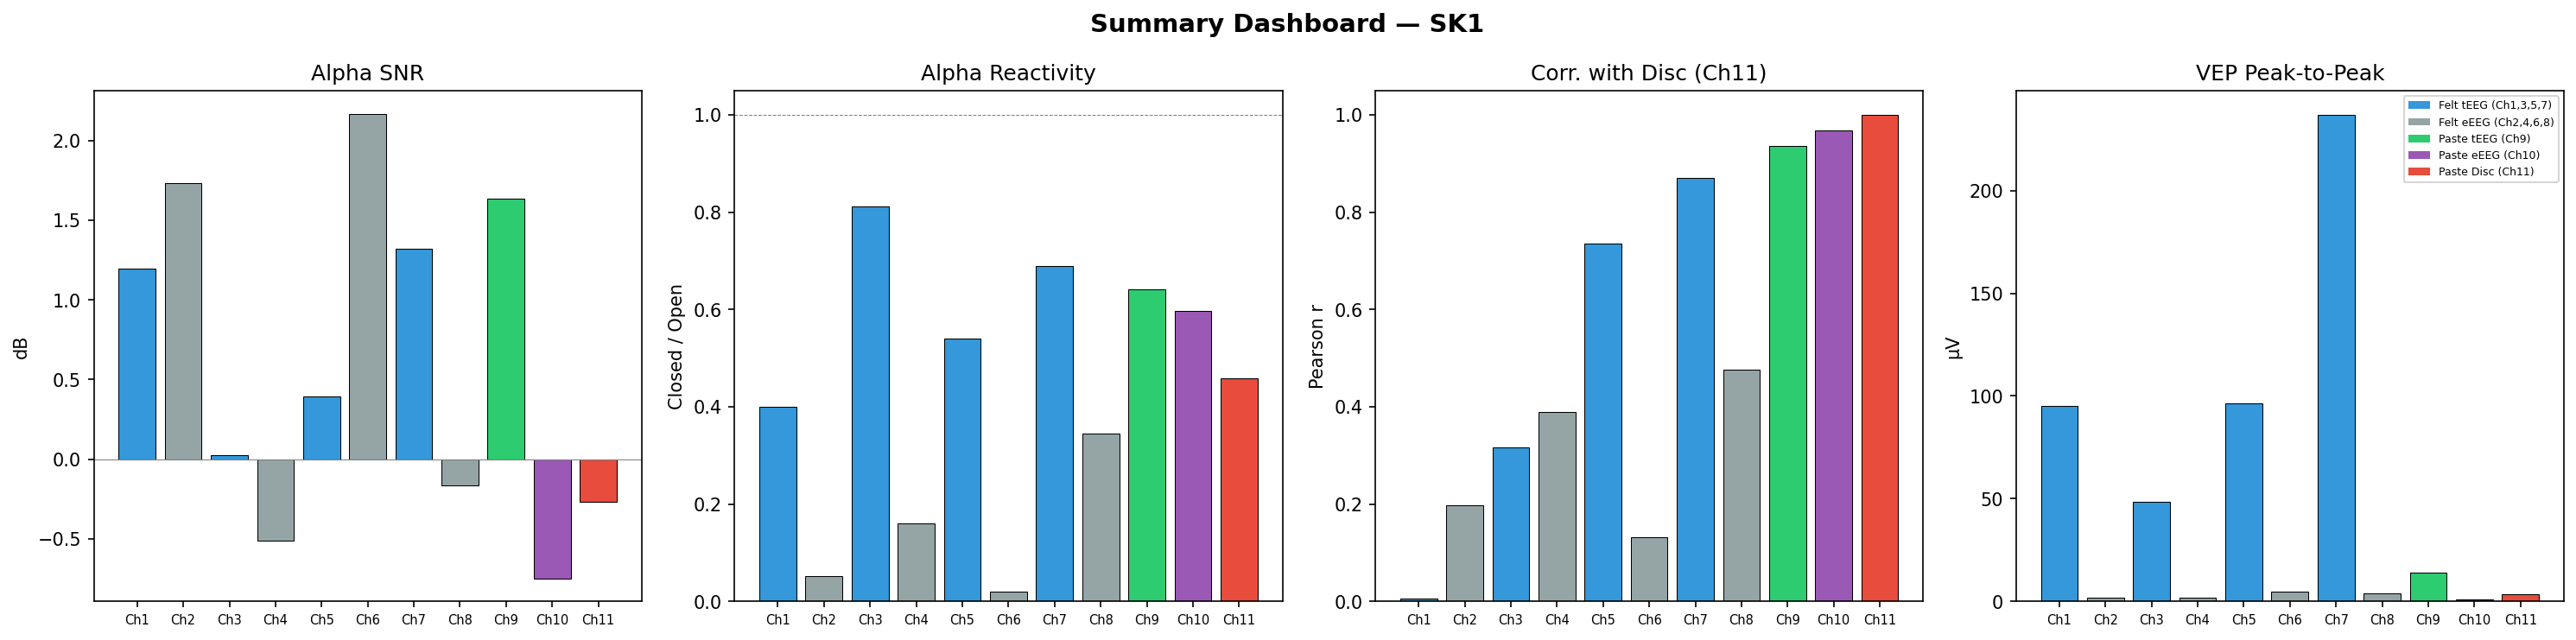
\includegraphics[width=\columnwidth]{fig_001.png}
  \caption{Summary dashboard: alpha SNR, reactivity (Closed/Open),
    disc correlation, and VEP amplitude per channel.}
  \label{fig:dashboard}
\end{figure}

% ─────────────────────────────────────────────────────────────────────────────
\section{Alpha Reactivity: Why It Is All Below 1}

Alpha reactivity is the ratio of eyes-closed to eyes-open alpha power.
A ratio above 1 means alpha goes up when you close your eyes -- that is
the Berger effect~\cite{kirschfeld2005}, and what we want to see.
Right now every channel is below 1, so open-eye alpha is actually higher,
which is backwards.

My best explanation is that the visual stimulation blocks (S7 events)
happened during open-eye periods, and on the clipping tEEG channels those
blocks inflated broadband power significantly.
So it is more of an artifact problem than a real neurological finding.
Ch3 came closest to the Berger threshold at 0.81$\times$, and among
non-clipping channels Ch9 was the best at 0.64$\times$.
Once the impedance issue is fixed I expect this will look a lot more like
what we want.

\begin{figure}[t]
  \centering
  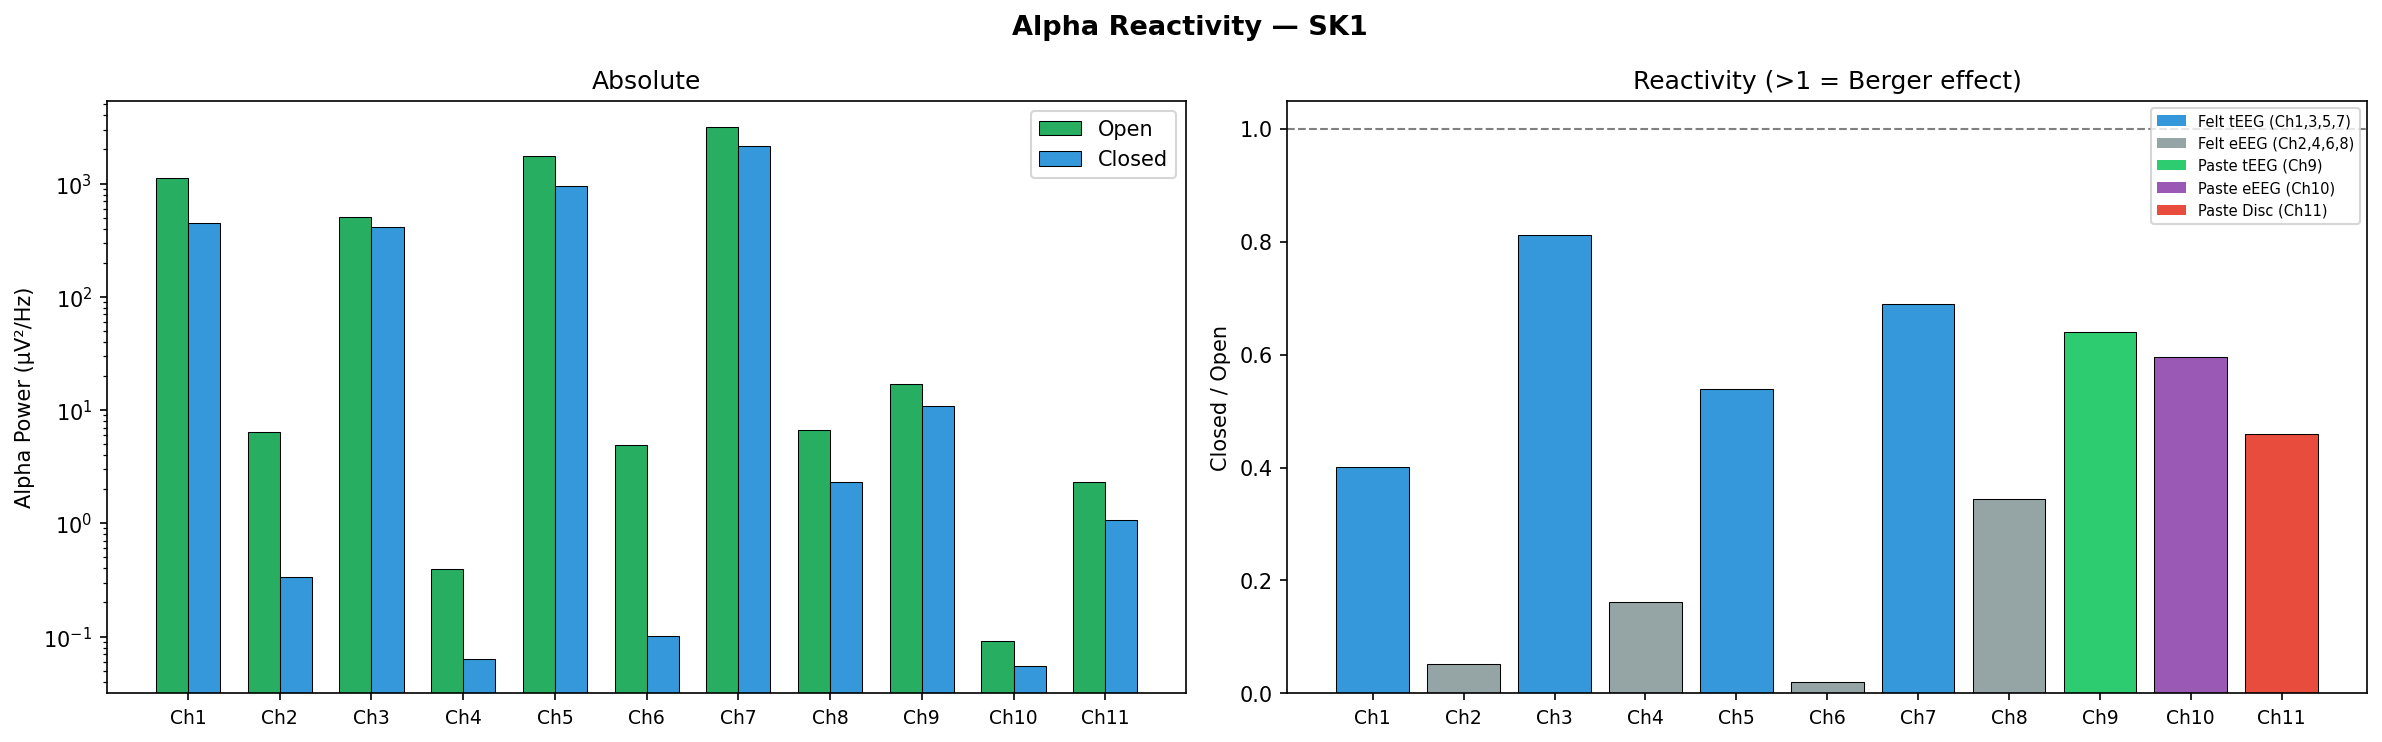
\includegraphics[width=\columnwidth]{fig_029.png}
  \caption{Alpha reactivity. Left: absolute alpha power open vs.\ closed.
    Right: Closed/Open ratio; dashed line at 1.0 marks the Berger threshold.}
  \label{fig:reactivity}
\end{figure}

% ─────────────────────────────────────────────────────────────────────────────
\section{Eyes-Open vs.\ Eyes-Closed PSD}

You mentioned the different y-axis scales make it hard to compare channels
directly -- the plots now use a shared normalized y-axis for easier comparison.
Even so, you can see alpha peaks around 10--13\,Hz in Ch9, Ch10, and Ch11
during eyes-closed, which is encouraging.
The full per-channel PSD plots are in Appendix\,\ref{app:psd}.

\begin{figure}[t]
  \centering
  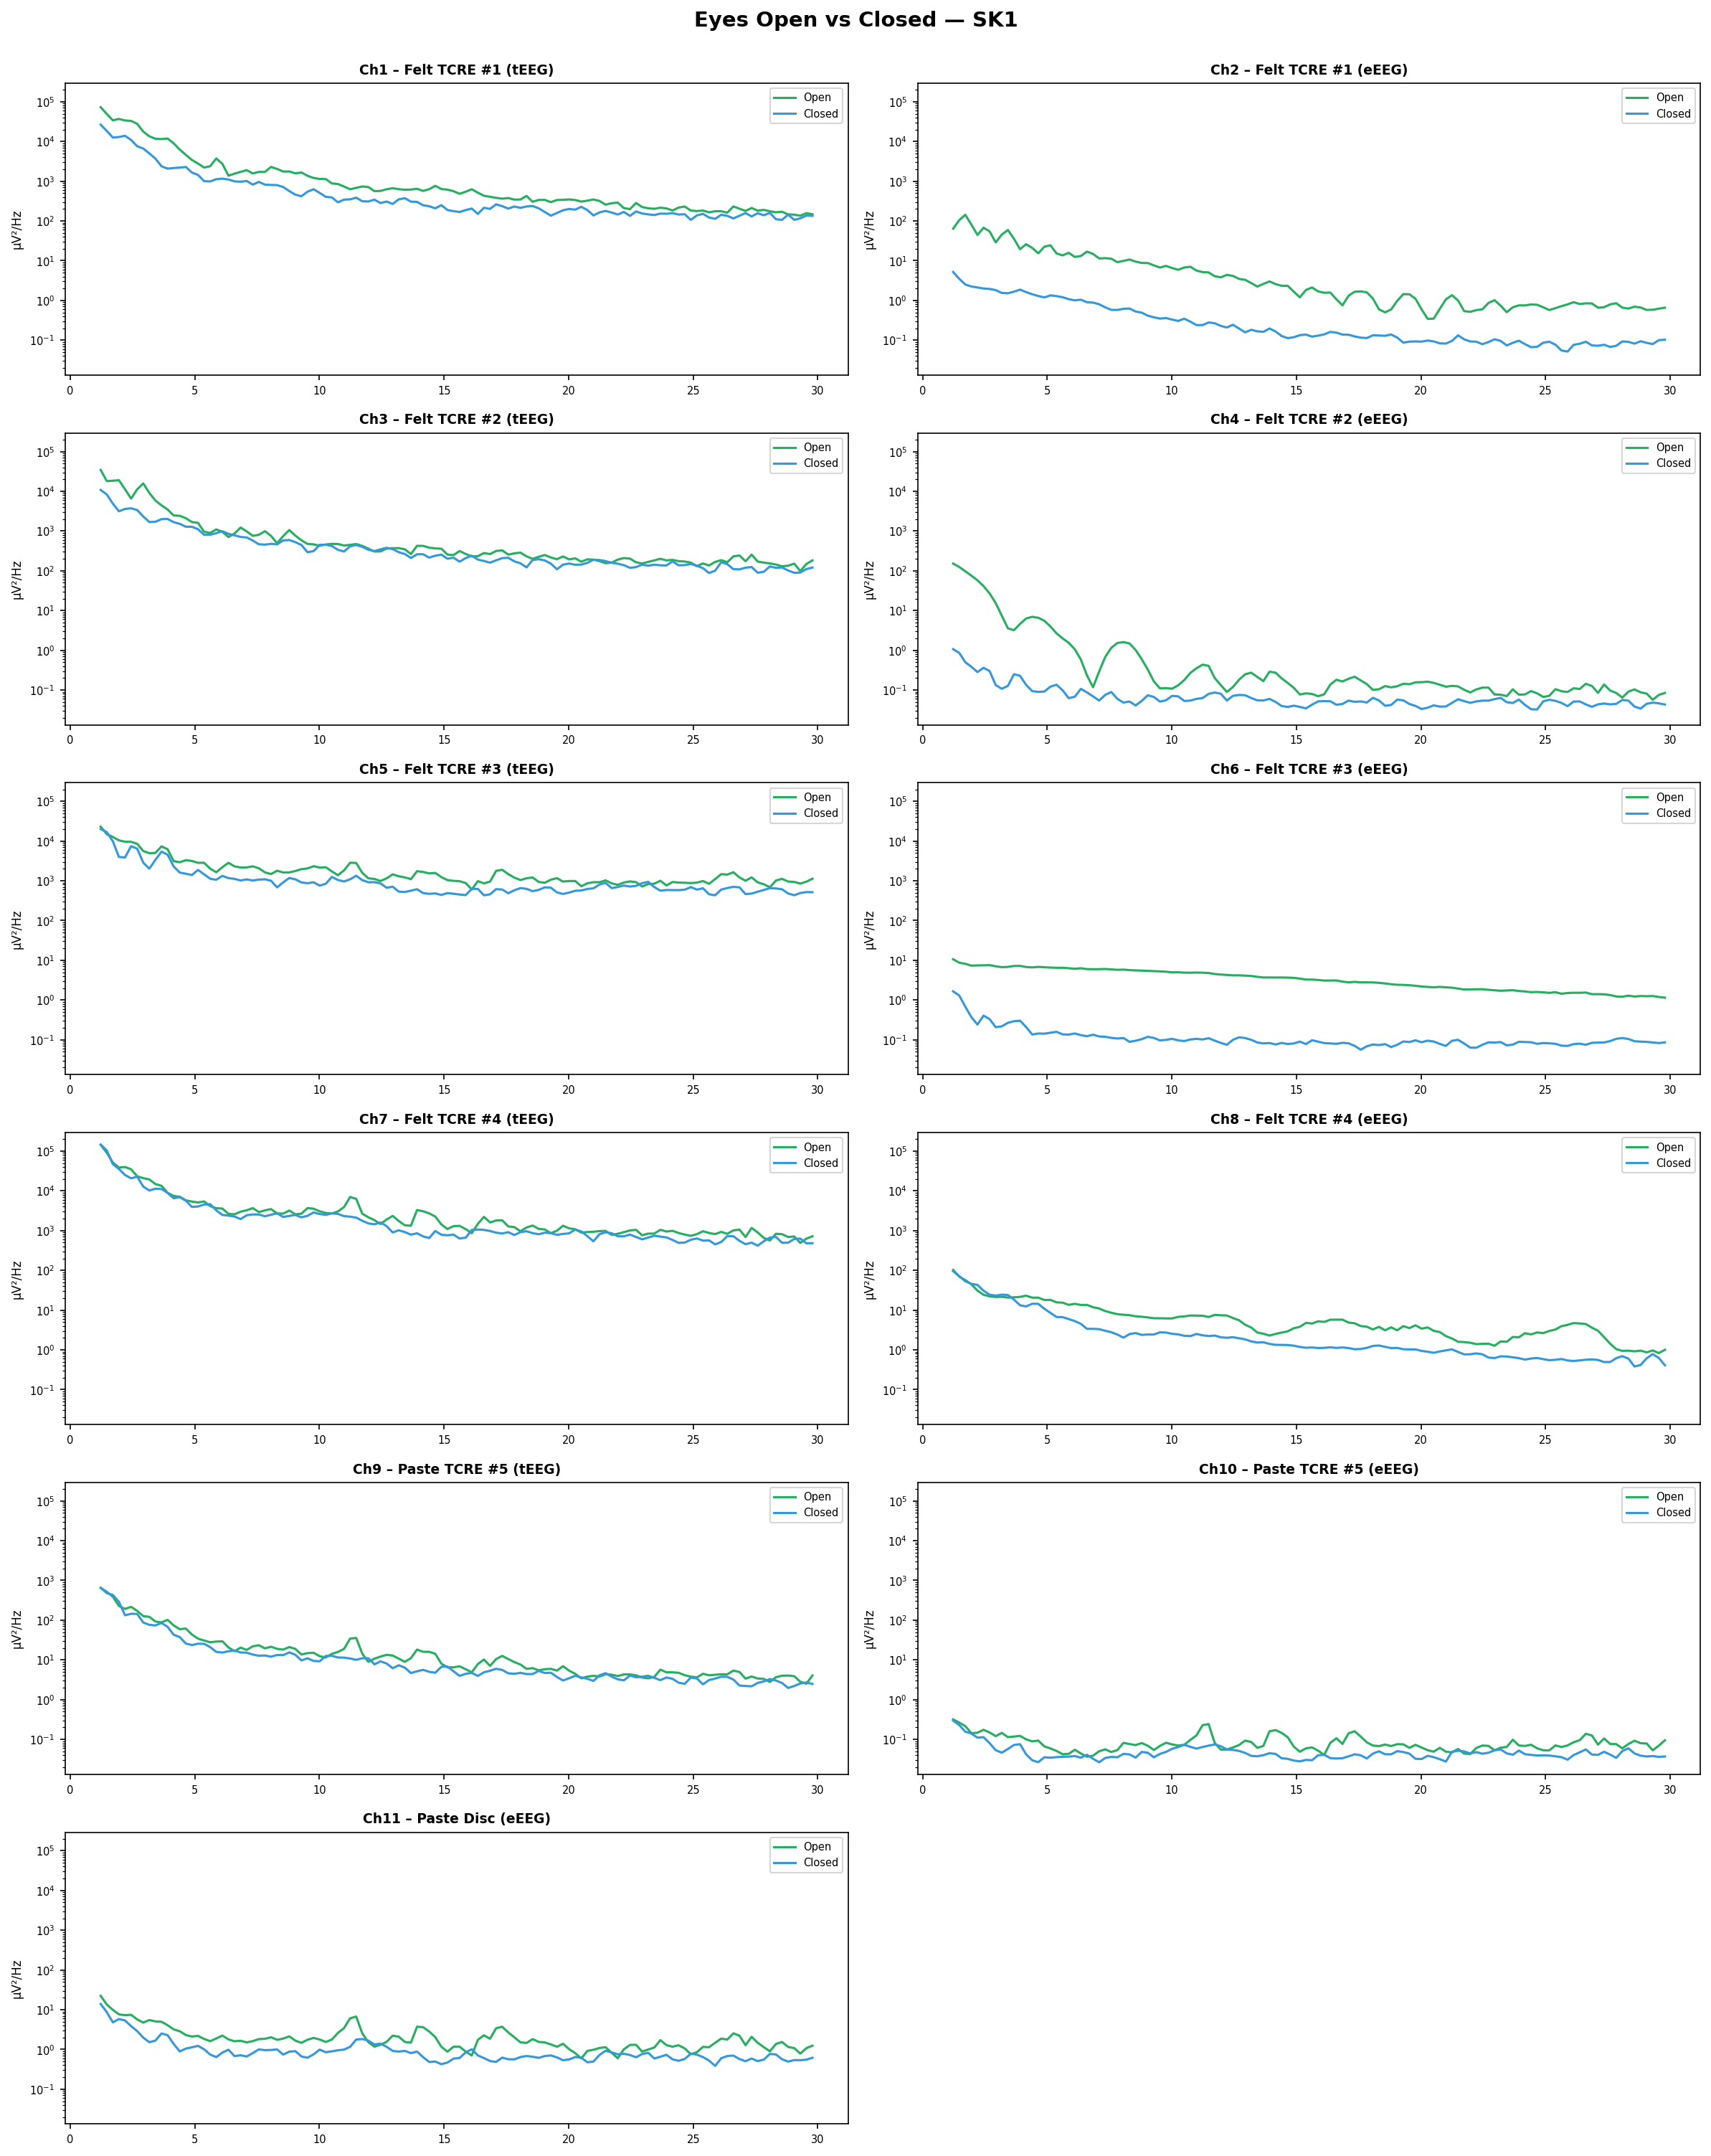
\includegraphics[width=\columnwidth]{fig_030.png}
  \caption{Eyes-open (green) vs.\ eyes-closed (blue) PSD per channel.
    Y-axis scales are normalized across channels for direct comparison.}
  \label{fig:psd}
\end{figure}

% ─────────────────────────────────────────────────────────────────────────────
\section{FOOOF Spectral Parameterization}

I ran the FOOOF (specparam) algorithm~\cite{donoghue2020} on each channel to separate the
oscillatory alpha peak from the aperiodic 1/f background.
Table\,\ref{tab:fooof} summarizes the results.

A few things to note.
An alpha peak was detected in only 5 of the 11 channels, which partly
reflects the clipping problem masking the alpha band on the felt tEEG
channels.
Ch9 (paste tEEG) and Ch10 (paste eEEG) both show clean alpha peaks around
12.7\,Hz and 10.8\,Hz respectively, which are the most trustworthy.
Ch10 and Ch11 have poor aperiodic fits ($R^{2} = 0.80$ and $0.02$) --
Ch11's fit is essentially useless, consistent with the clipping making its
spectrum nonstationary, and Ch10 has an unusual rising high-frequency tail
that FOOOF struggles with.

\begin{table*}[t]
  \centering
  \caption{FOOOF spectral parameterization results for subject SK1.
    Channels with no detected alpha peak had no clear oscillatory
    component above the 1/f background.}
  \label{tab:fooof}
  \renewcommand{\arraystretch}{1.2}
  \begin{tabular}{llccrrc}
    \toprule
    \textbf{Channel} & \textbf{Type} &
    \textbf{$\alpha$ Peak (Hz)} & \textbf{Amplitude} &
    \textbf{Aperiodic Offset} & \textbf{Slope} &
    \textbf{$R^{2}$} \\
    \midrule
    Ch1  & Felt tEEG \#1  &  8.60 & 0.12 &  4.77 &  1.79 & 0.97 \\
    Ch2  & Felt eEEG \#1  & --    & --   &  1.78 &  1.63 & 0.99 \\
    Ch3  & Felt tEEG \#2  & --    & --   &  4.21 &  1.34 & 1.00 \\
    Ch4  & Felt eEEG \#2  & --    & --   &  1.40 &  1.60 & 0.99 \\
    Ch5  & Felt tEEG \#3  & --    & --   &  3.72 &  0.50 & 0.97 \\
    Ch6  & Felt eEEG \#3  & 12.97 & 0.16 &  1.08 &  0.65 & 0.98 \\
    Ch7  & Felt tEEG \#4  & 11.14 & 0.12 &  4.88 &  1.33 & 0.90 \\
    Ch8  & Felt eEEG \#4  & --    & --   &  2.53 &  1.79 & 0.97 \\
    Ch9  & Paste tEEG \#5 & 12.70 & 0.17 &  2.57 &  1.28 & 0.93 \\
    Ch10 & Paste eEEG \#5 & 10.81 & 0.20 & -1.64 & -0.53 & 0.80\textsuperscript{*} \\
    Ch11 & Paste Disc     & 12.77 & 0.23 &  0.40 &  0.01 & 0.02\textsuperscript{*} \\
    \bottomrule
    \multicolumn{7}{l}{\small \textsuperscript{*} Poor aperiodic fit -- interpret with caution.}
  \end{tabular}
\end{table*}

% ─────────────────────────────────────────────────────────────────────────────
\section{Correlation with the Disc}

This one is actually reassuring rather than a problem.
Fig.\,\ref{fig:corr} shows how strongly each channel's alpha envelope tracks
the paste disc (Ch11).
The paste eEEG (Ch10, $r=0.968$) and paste tEEG (Ch9, $r=0.936$) track it
very closely, as expected.
The felt tEEG Laplacian channels have much lower correlation -- Ch1 is
almost zero ($r=0.006$).

That low number is not the Laplacian failing; it is the Laplacian working.
The Laplacian derivation suppresses the broadly distributed alpha field that
the disc picks up and captures more local cortical activity instead.
So the divergence from the disc is expected and is actually one of the key
things the TCRE is supposed to do.

\begin{figure}[t]
  \centering
  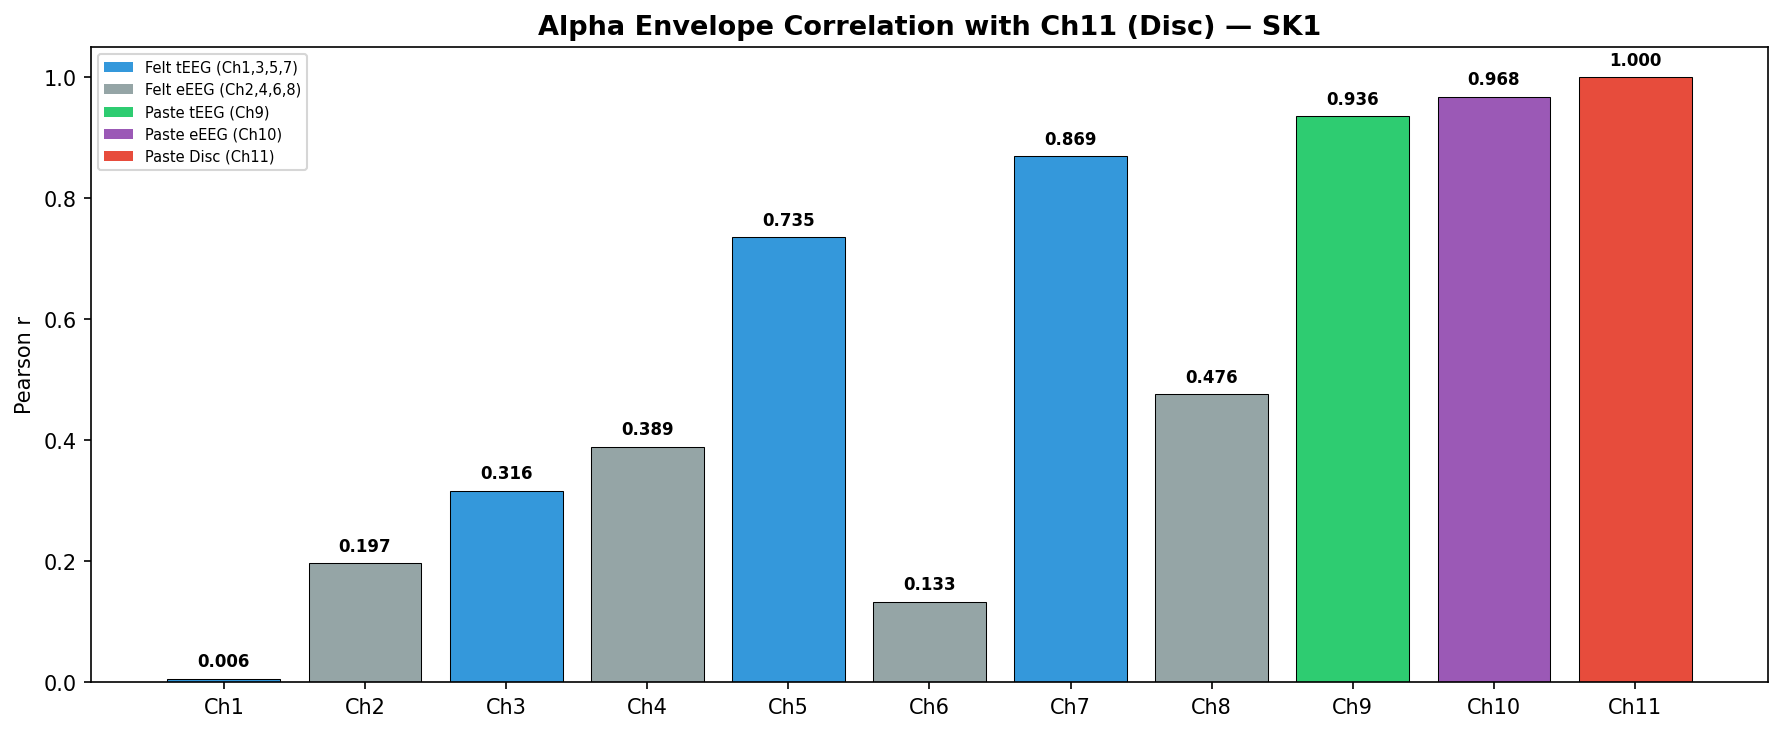
\includegraphics[width=\columnwidth]{fig_032.png}
  \caption{Pearson correlation of each channel's alpha envelope with Ch11
    (disc). Low tEEG values reflect spatial filtering, not signal loss.}
  \label{fig:corr}
\end{figure}

% ─────────────────────────────────────────────────────────────────────────────
\section{Visual Evoked Potentials}

Fig.\,\ref{fig:vep} shows the VEP grand averages across 74 trials.
The biggest number is Ch7 at 236.8\,$\mu$V, which is almost certainly noise
from the high impedance rather than a real VEP.
The most trustworthy VEP is Ch9 (paste tEEG) at 13.9\,$\mu$V -- clean
signal, no clipping, reasonable amplitude.
The disc and eEEG channels are all under 5\,$\mu$V, consistent with the
Laplacian being better at resolving focal evoked responses.

\begin{figure}[t]
  \centering
  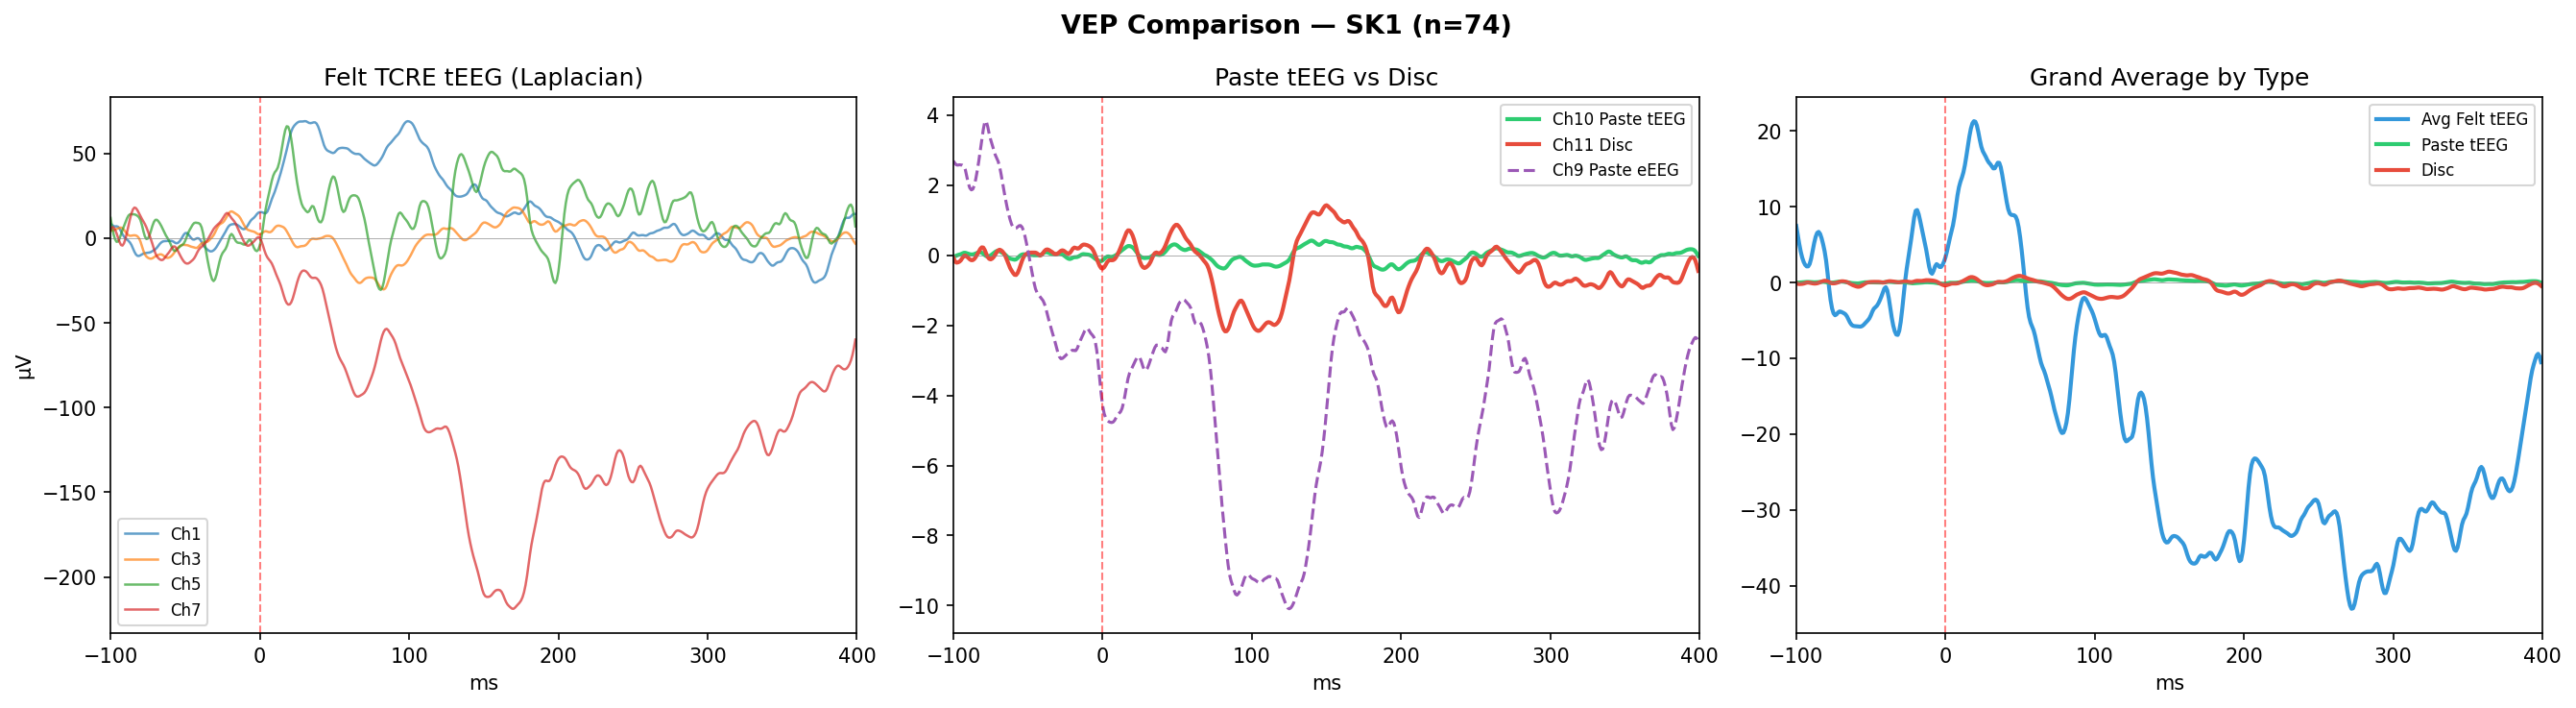
\includegraphics[width=\columnwidth]{fig_031.png}
  \caption{VEP comparison (74 trials). Left: felt tEEG channels.
    Center: paste channels vs.\ disc.
    Right: grand average by electrode type.}
  \label{fig:vep}
\end{figure}

% ─────────────────────────────────────────────────────────────────────────────
\section{Spectrogram SSIM: Image Comparison Between tEEG and eEEG}

This is the image processing comparison you suggested.
For each TCRE pair, I computed SSIM~\cite{wang2004} between the tEEG and eEEG spectrograms.
An SSIM of 1.0 means identical; 0.8+ is high similarity.
All five pairs came out between 0.32 and 0.48, so there is real structural
divergence -- the Laplacian is genuinely changing the time-frequency
structure of the signal, not just scaling it.

Table\,\ref{tab:ssim} summarizes the scores and
Figs.\,\ref{fig:ssim1}--\ref{fig:ssim5} show the full triplet comparisons.
The difference maps are uniformly positive (tEEG\,$>$\,eEEG in power), which
on the felt pairs reflects the noise inflation from high impedance.
On the paste pair (Fig.\,\ref{fig:ssim5}), the difference is smooth and
spread evenly, which is what spatial filtering should actually look like.
That gives me confidence this comparison will be much cleaner once we fix
the impedance issue on the felt electrodes.

\begin{table}[t]
  \centering
  \caption{Spectrogram SSIM scores per TCRE pair.}
  \label{tab:ssim}
  \renewcommand{\arraystretch}{1.2}
  \begin{tabular}{lc}
    \toprule
    \textbf{TCRE Pair} & \textbf{SSIM} \\
    \midrule
    Felt TCRE \#1 (Ch1/Ch2)   & 0.379 \\
    Felt TCRE \#2 (Ch3/Ch4)   & 0.321 \\
    Felt TCRE \#3 (Ch5/Ch6)   & 0.482 \\
    Felt TCRE \#4 (Ch7/Ch8)   & 0.417 \\
    Paste TCRE \#5 (Ch9/Ch10) & 0.400 \\
    \bottomrule
  \end{tabular}
\end{table}

\begin{figure}[t]
  \centering
  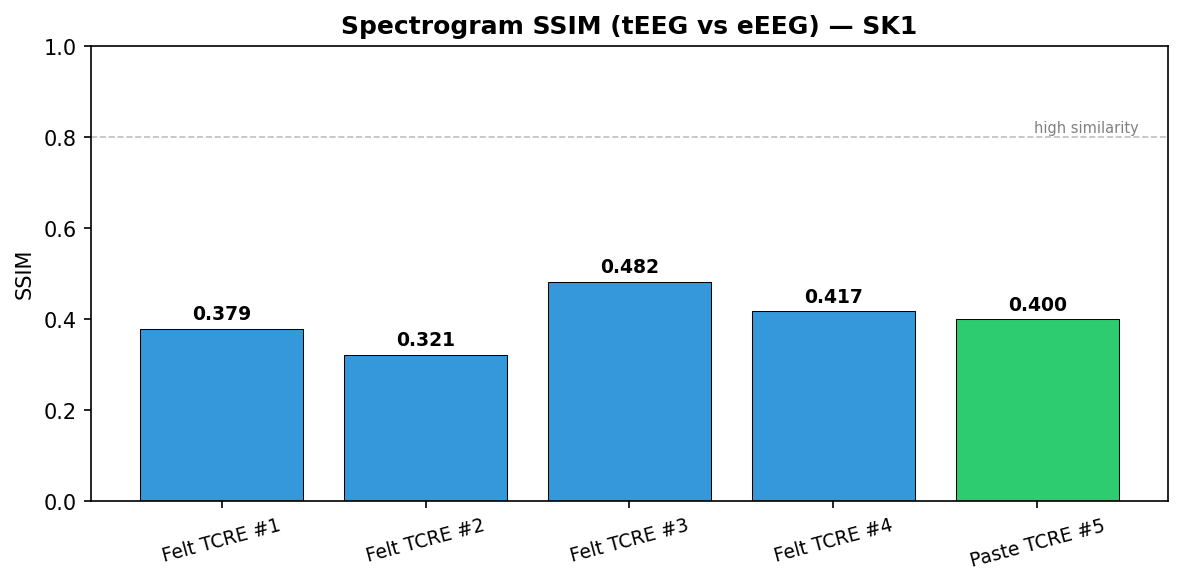
\includegraphics[width=0.82\columnwidth]{fig_038.png}
  \caption{SSIM bar chart per TCRE pair. All values $<0.8$ confirm
    meaningful structural divergence between Laplacian and conventional
    derivations.}
  \label{fig:ssim_bar}
\end{figure}

\begin{figure*}[t]
  \centering
  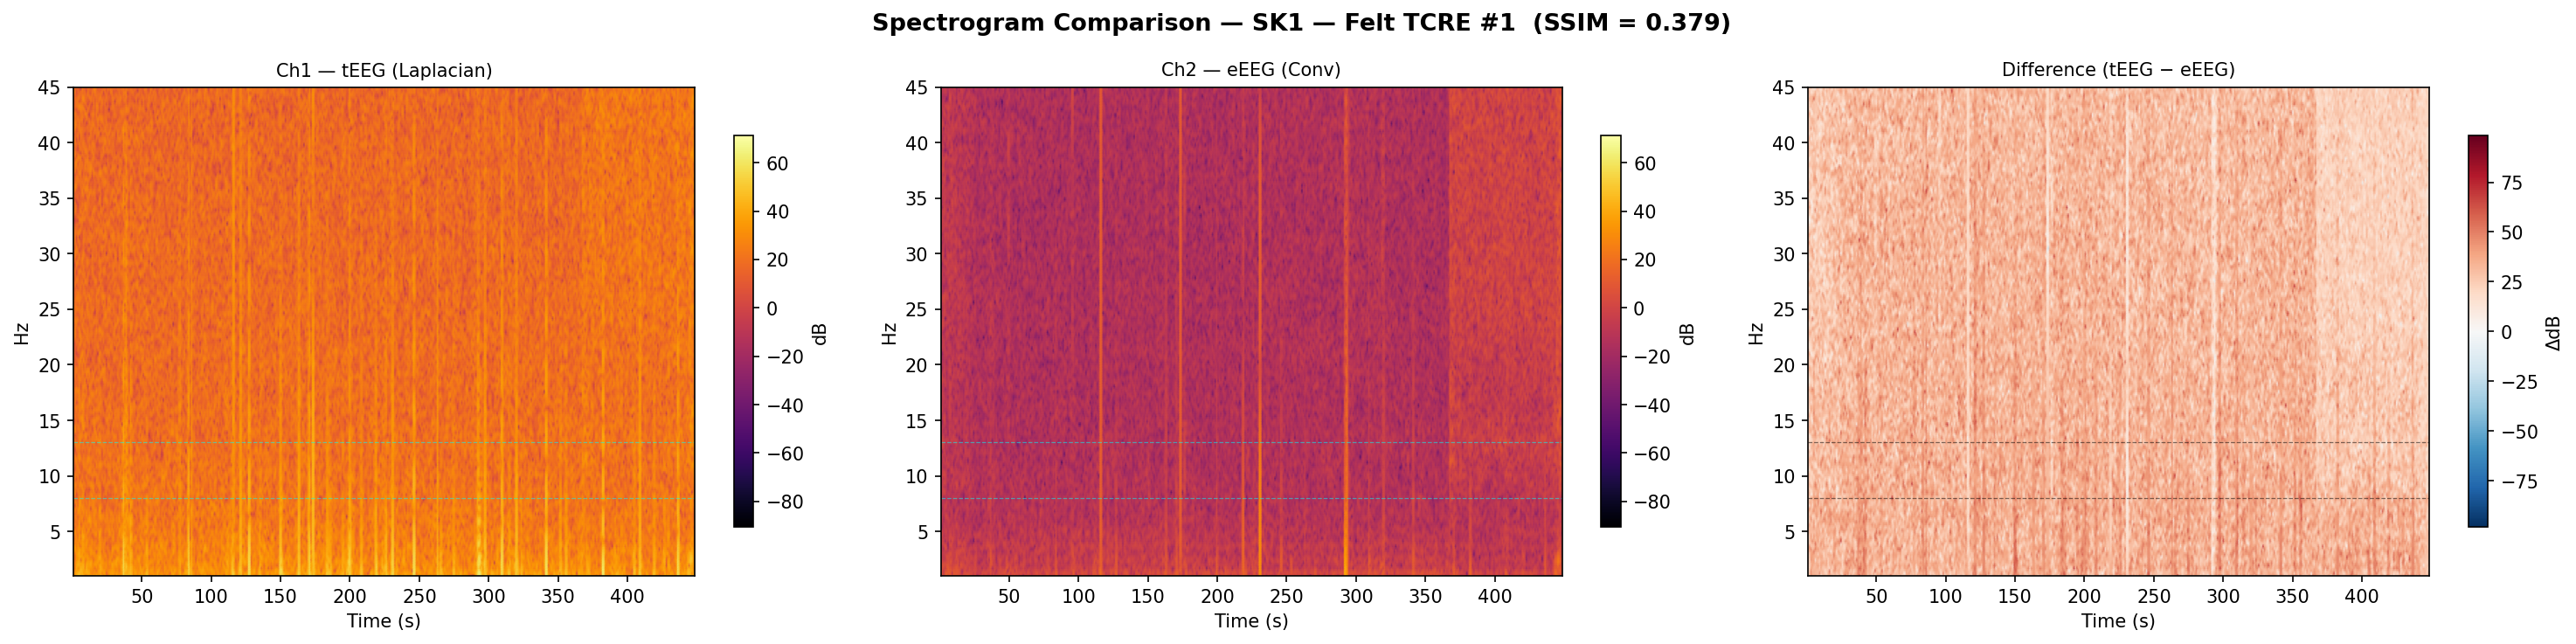
\includegraphics[width=\textwidth]{fig_033.png}
  \caption{Felt TCRE\,\#1 (Ch1/Ch2), SSIM\,=\,0.379. tEEG has higher
    broadband power throughout.}
  \label{fig:ssim1}
\end{figure*}

\begin{figure*}[t]
  \centering
  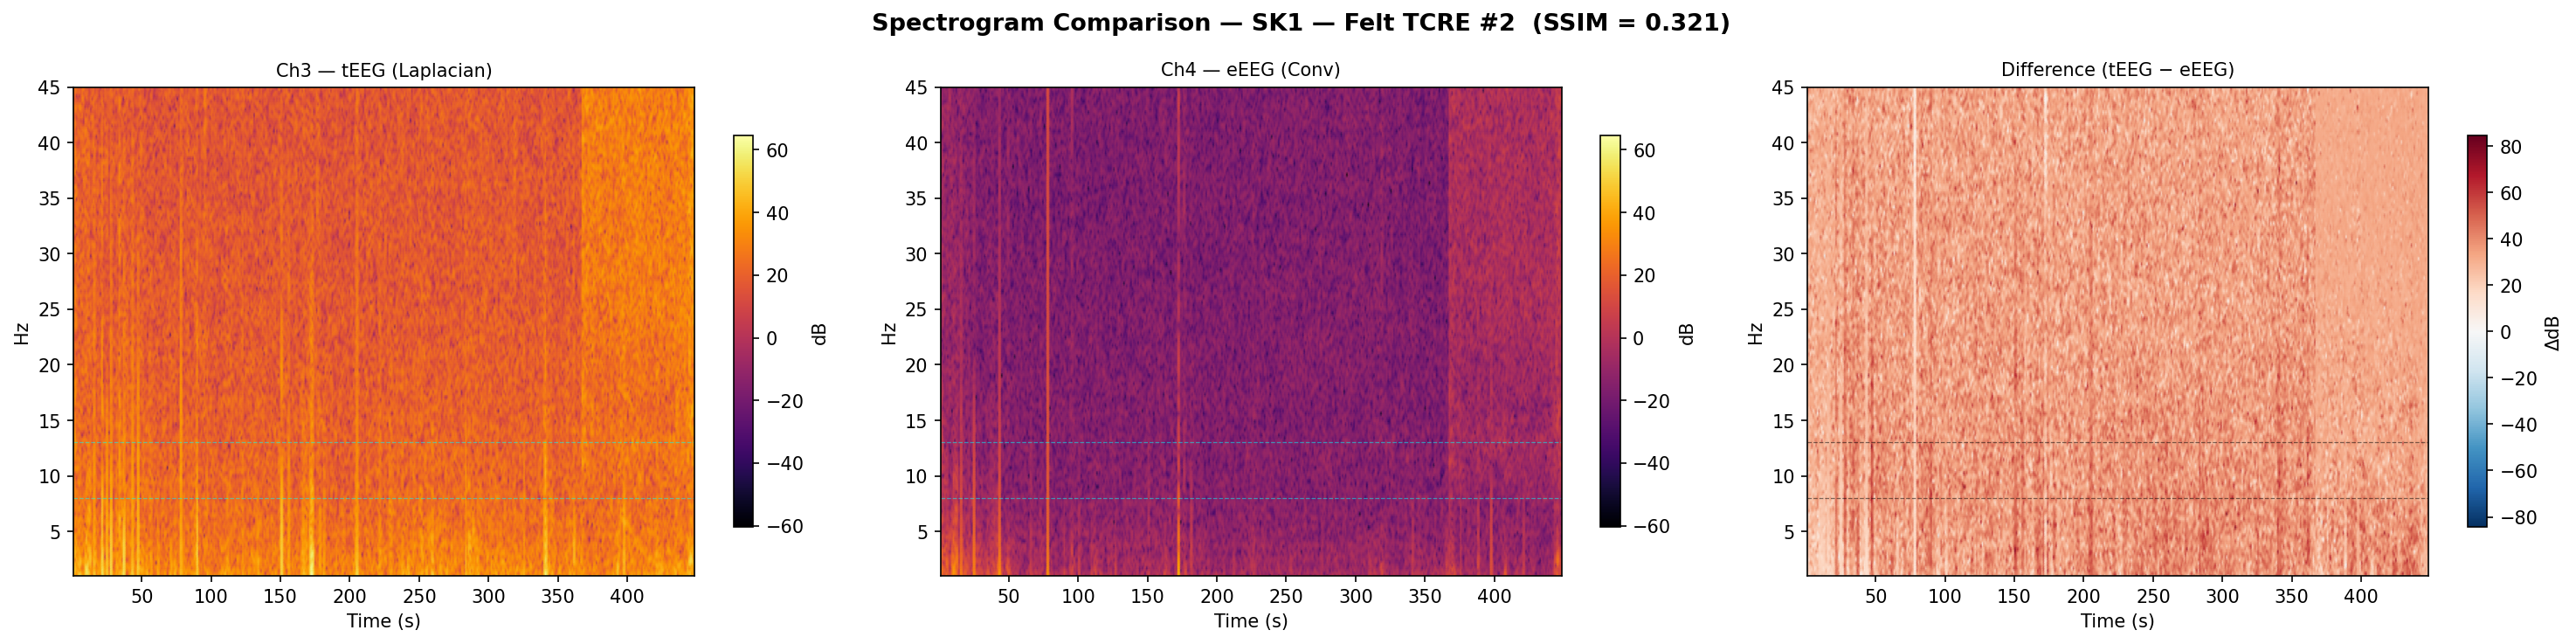
\includegraphics[width=\textwidth]{fig_034.png}
  \caption{Felt TCRE\,\#2 (Ch3/Ch4), SSIM\,=\,0.321. Largest divergence;
    eEEG shows a signal drop around 375\,s.}
  \label{fig:ssim2}
\end{figure*}

\begin{figure*}[t]
  \centering
  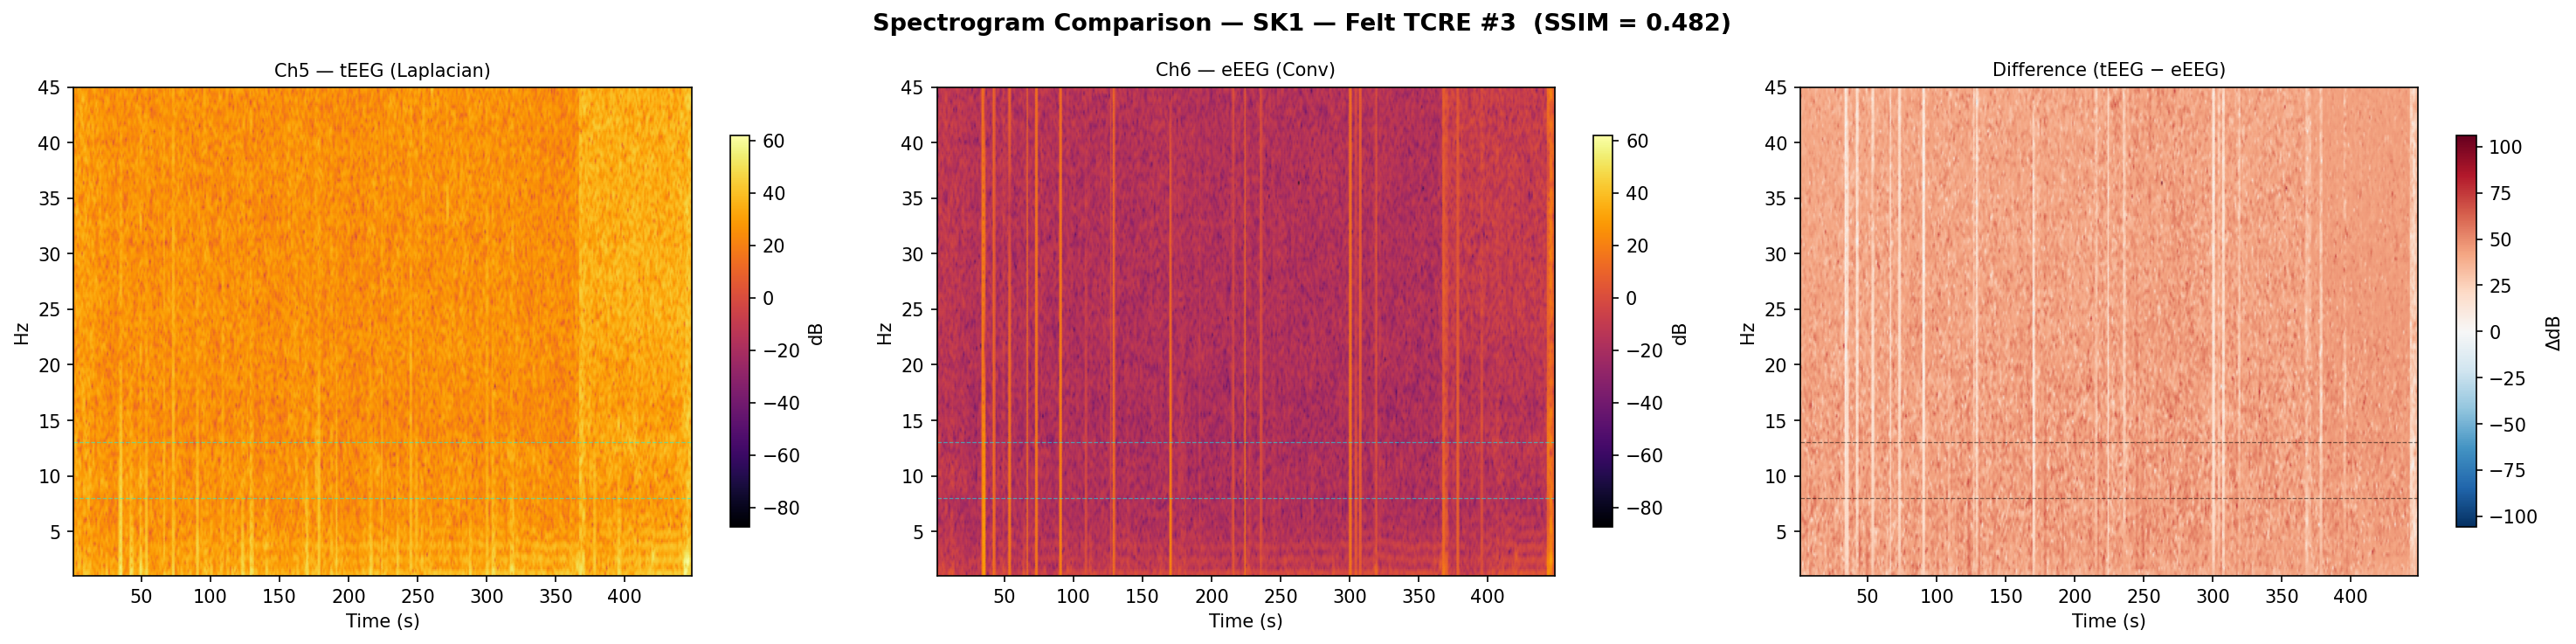
\includegraphics[width=\textwidth]{fig_035.png}
  \caption{Felt TCRE\,\#3 (Ch5/Ch6), SSIM\,=\,0.482. Most similar pair --
    both channels mostly dominated by broadband noise at this point.}
  \label{fig:ssim3}
\end{figure*}

\begin{figure*}[t]
  \centering
  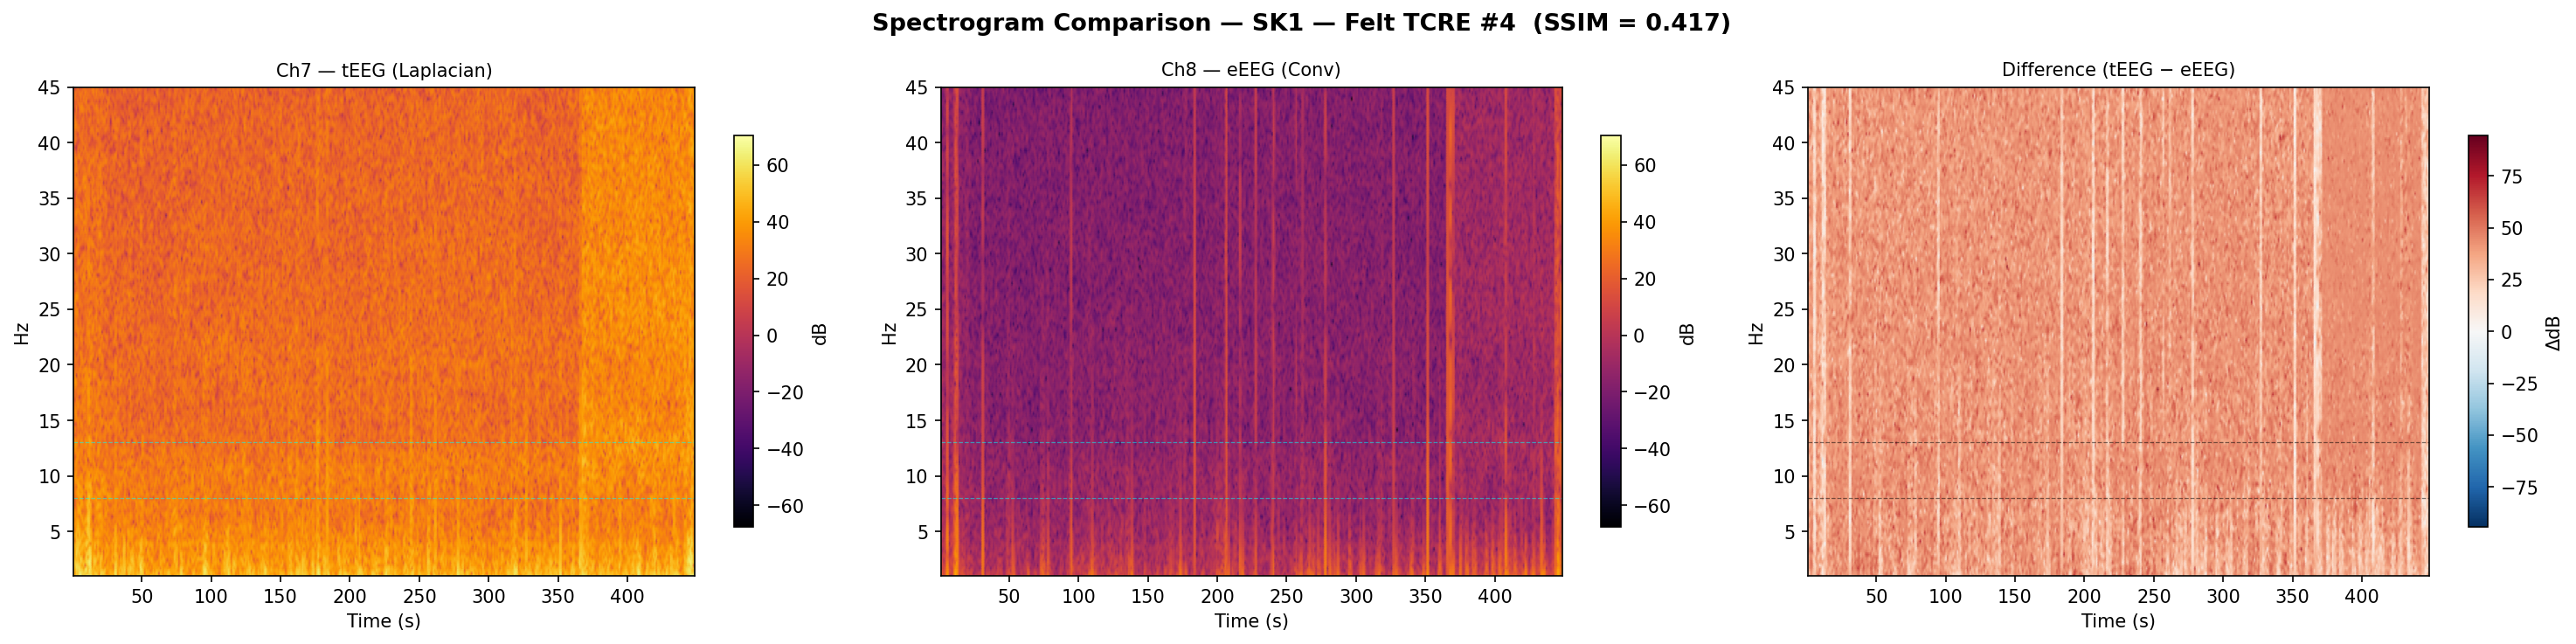
\includegraphics[width=\textwidth]{fig_036.png}
  \caption{Felt TCRE\,\#4 (Ch7/Ch8), SSIM\,=\,0.417. eEEG shows large
    impulse artifacts absent from the tEEG Laplacian output.}
  \label{fig:ssim4}
\end{figure*}

\begin{figure*}[t]
  \centering
  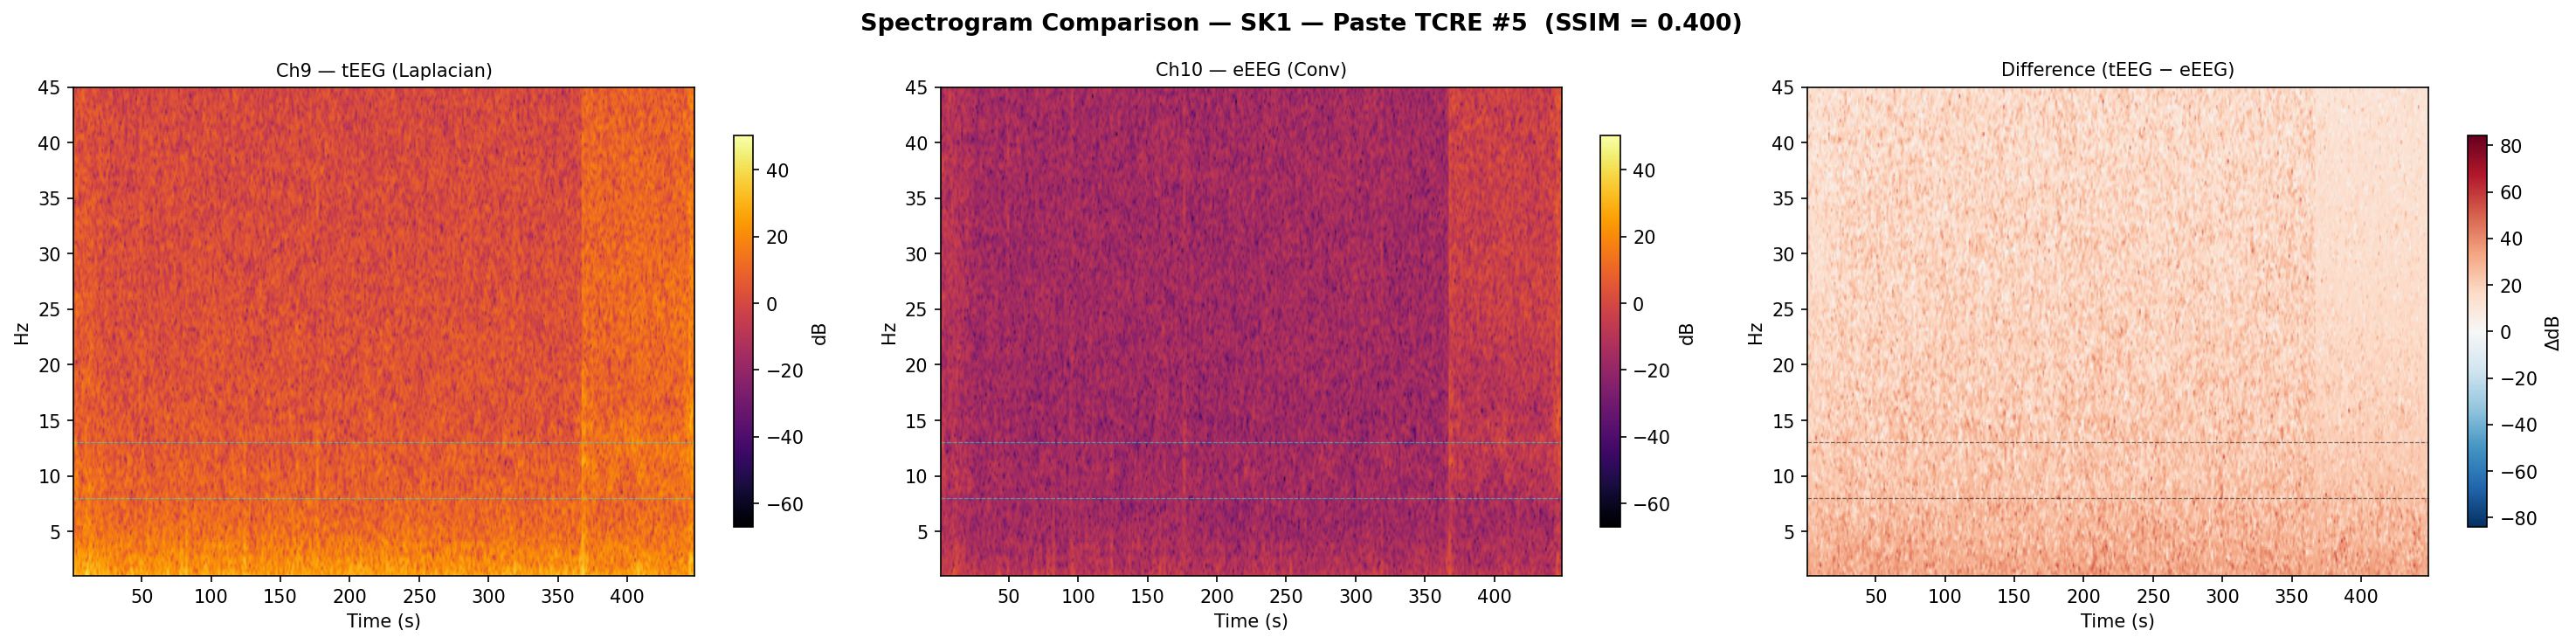
\includegraphics[width=\textwidth]{fig_037.png}
  \caption{Paste TCRE\,\#5 (Ch9/Ch10), SSIM\,=\,0.400. Cleanest pair;
    difference is smooth and uniform, consistent with spatial filtering
    rather than noise inflation.}
  \label{fig:ssim5}
\end{figure*}

% ─────────────────────────────────────────────────────────────────────────────
\section{What's Next}

\begin{itemize}
  \item Check electrode impedances before every future session --
        top priority.
  \item Start recording the remaining subjects and run the same pipeline
        on each.
  \item Once we have 5+ subjects with clean data, run the Wilcoxon
        signed-rank test to statistically compare SNR and reactivity
        between electrode types.
  \item Happy to set up a Zoom to walk through any of this in more
        detail -- just let me know what works.
\end{itemize}

% ─────────────────────────────────────────────────────────────────────────────
%  APPENDIX
% ─────────────────────────────────────────────────────────────────────────────
\appendices

\section{PSD After 60 Hz Notch: All Channels}
\label{app:psd}

Fig.\,\ref{fig:psd_all} shows the full Welch PSD~\cite{welch1967} for all 11 channels after
the 60\,Hz notch filter.
The orange shaded region marks the alpha band (8--13\,Hz).
Where a FOOOF peak was detected, the peak frequency is marked with a red
dashed line.
The tEEG channels have a much steeper 1/f slope and higher overall power
than their paired eEEG channels, which is the expected effect of the
Laplacian derivation reducing the common-mode signal.

\begin{figure*}[h]
  \centering
  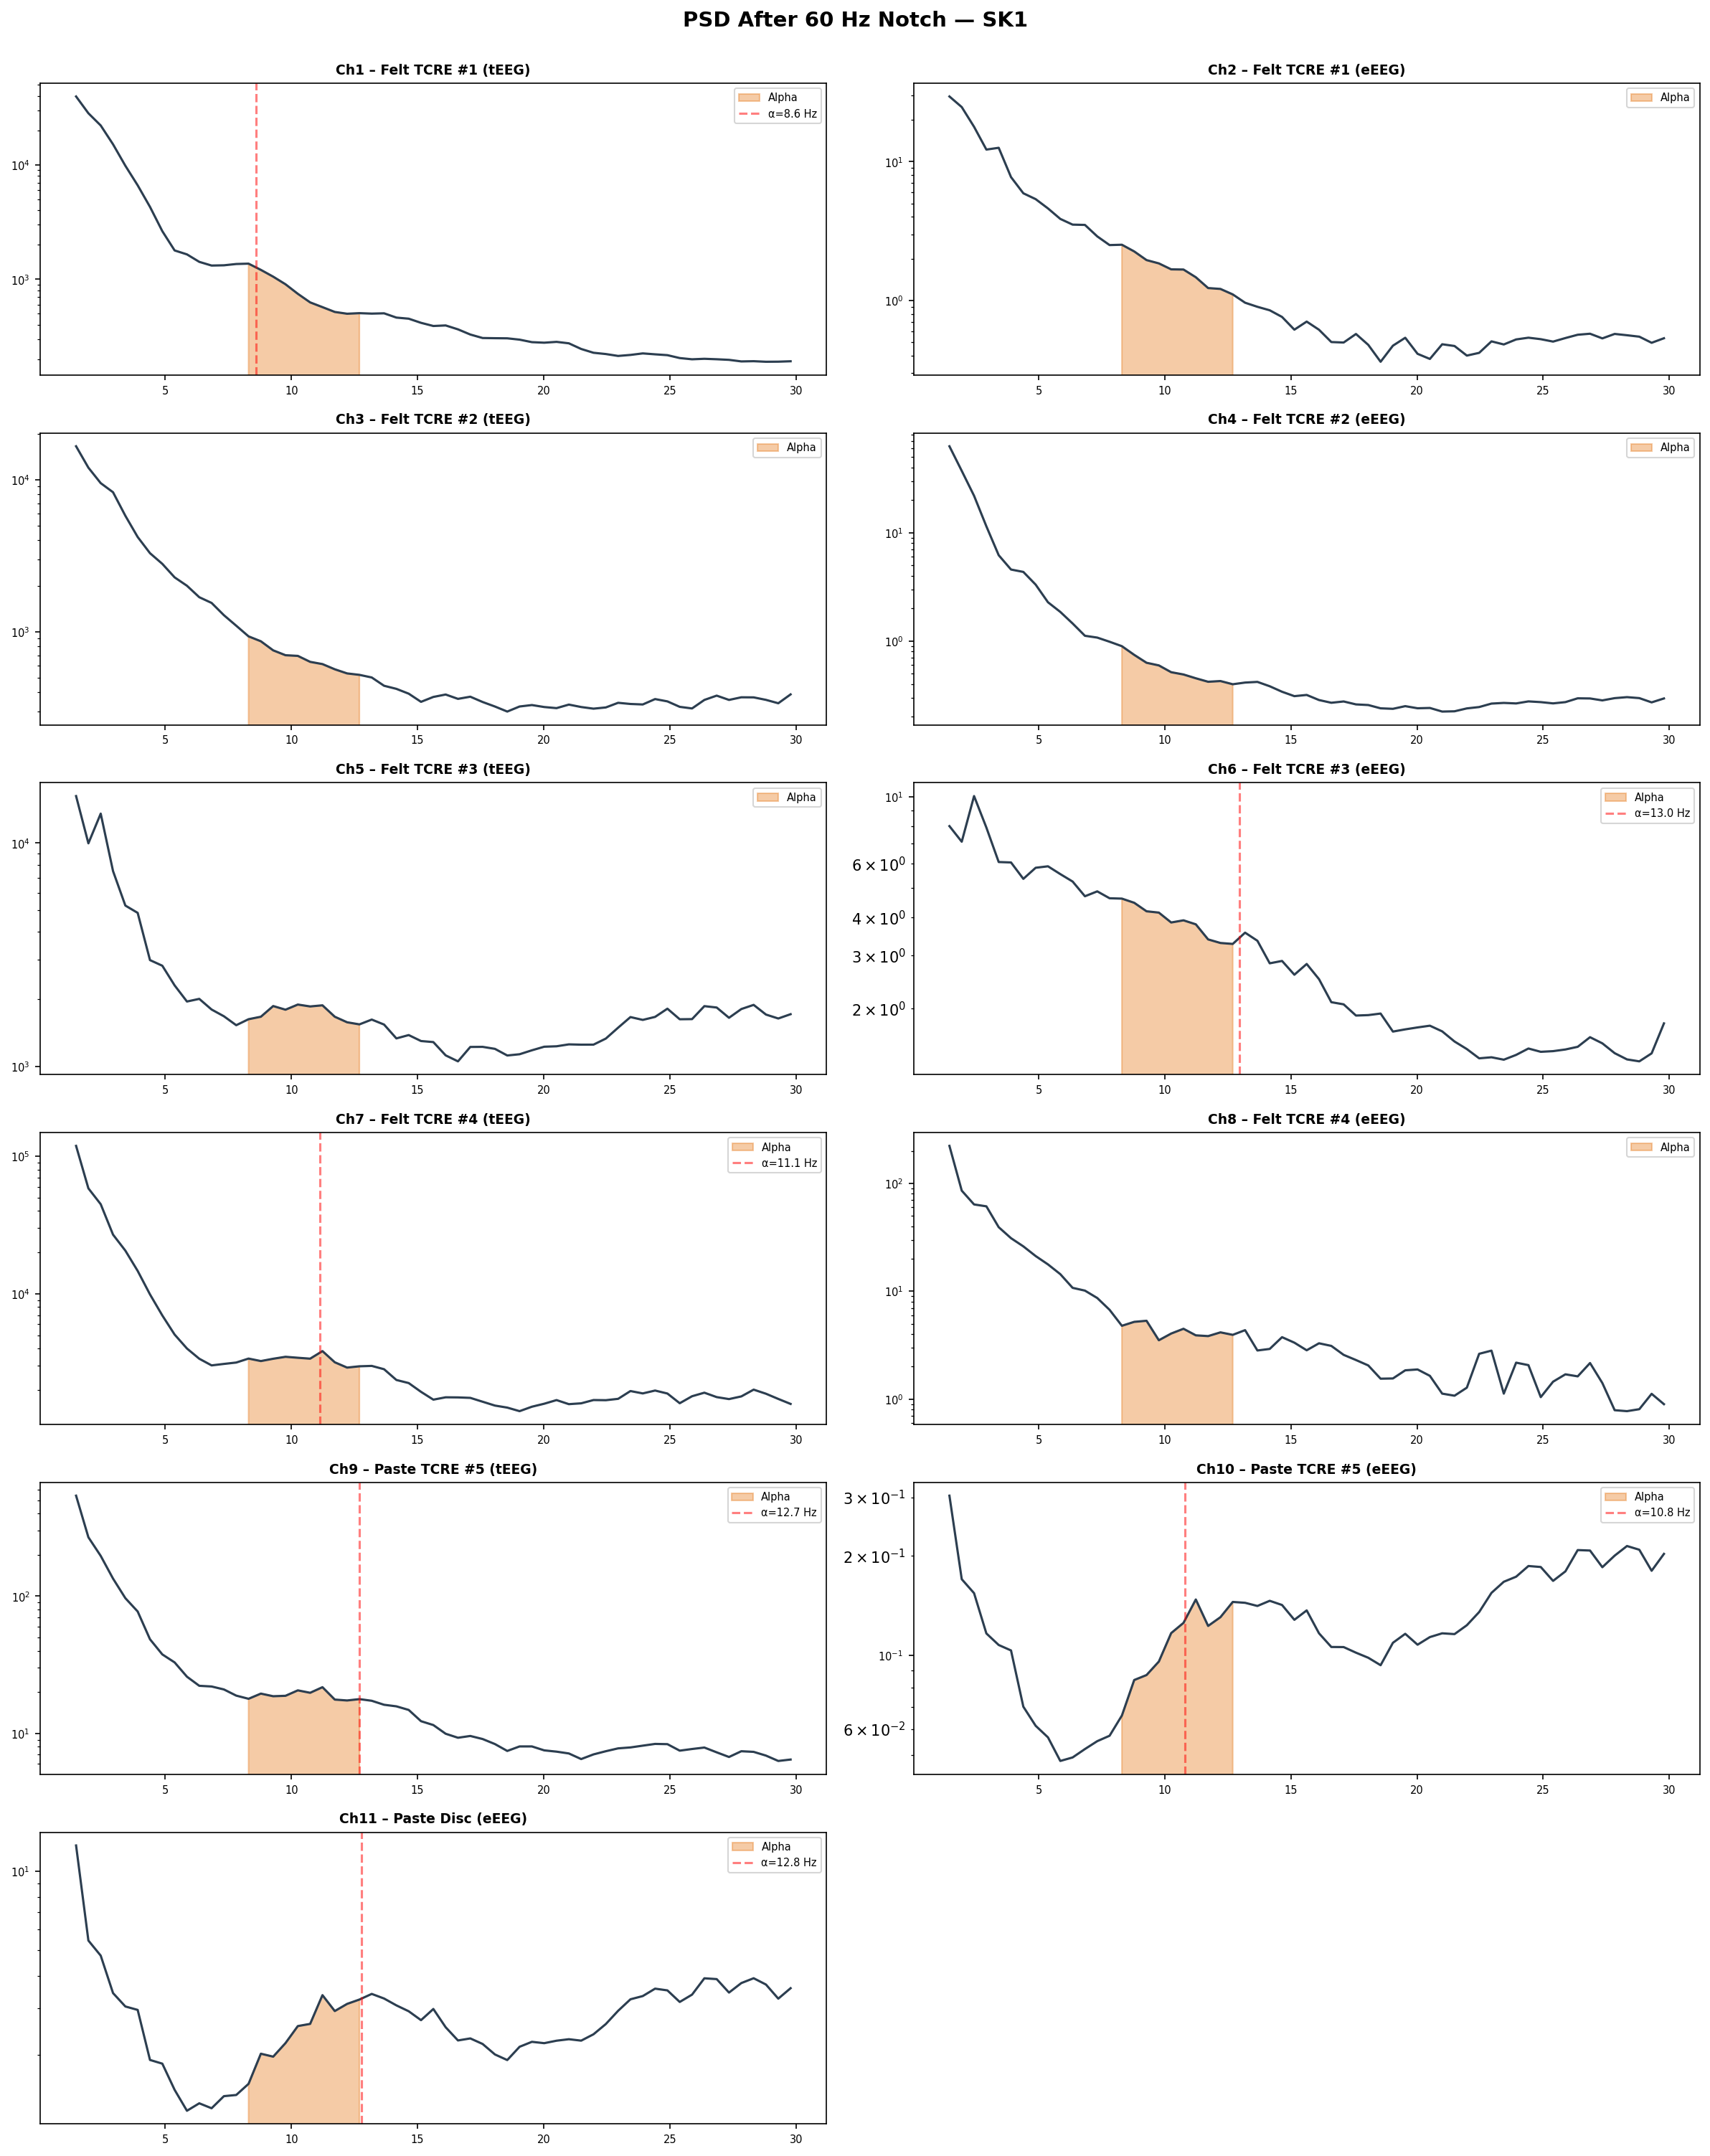
\includegraphics[width=0.72\textwidth]{fig_005.png}
  \caption{PSD (Welch, 0--30\,Hz) for all 11 channels after 60\,Hz notch
    filtering. Orange shading = alpha band (8--13\,Hz); red dashed line =
    FOOOF-detected alpha peak frequency where applicable.}
  \label{fig:psd_all}
\end{figure*}

\section{Per-Channel Spectrograms}
\label{app:spectrograms}

Figs.\,\ref{fig:spec_ch1}--\ref{fig:spec_ch11} show the time-frequency
spectrograms for each channel individually.
Each figure includes the raw EEG trace on top for reference.
Pink shaded regions are visual stimulation blocks (S7 events); light blue
shaded regions are the eyes-open/closed resting-state paradigm, with
``Open'' and ``Closed'' labels marking each transition.
The dashed cyan lines mark the alpha band boundaries (8 and 13\,Hz).

\begin{figure*}[h]
  \centering
  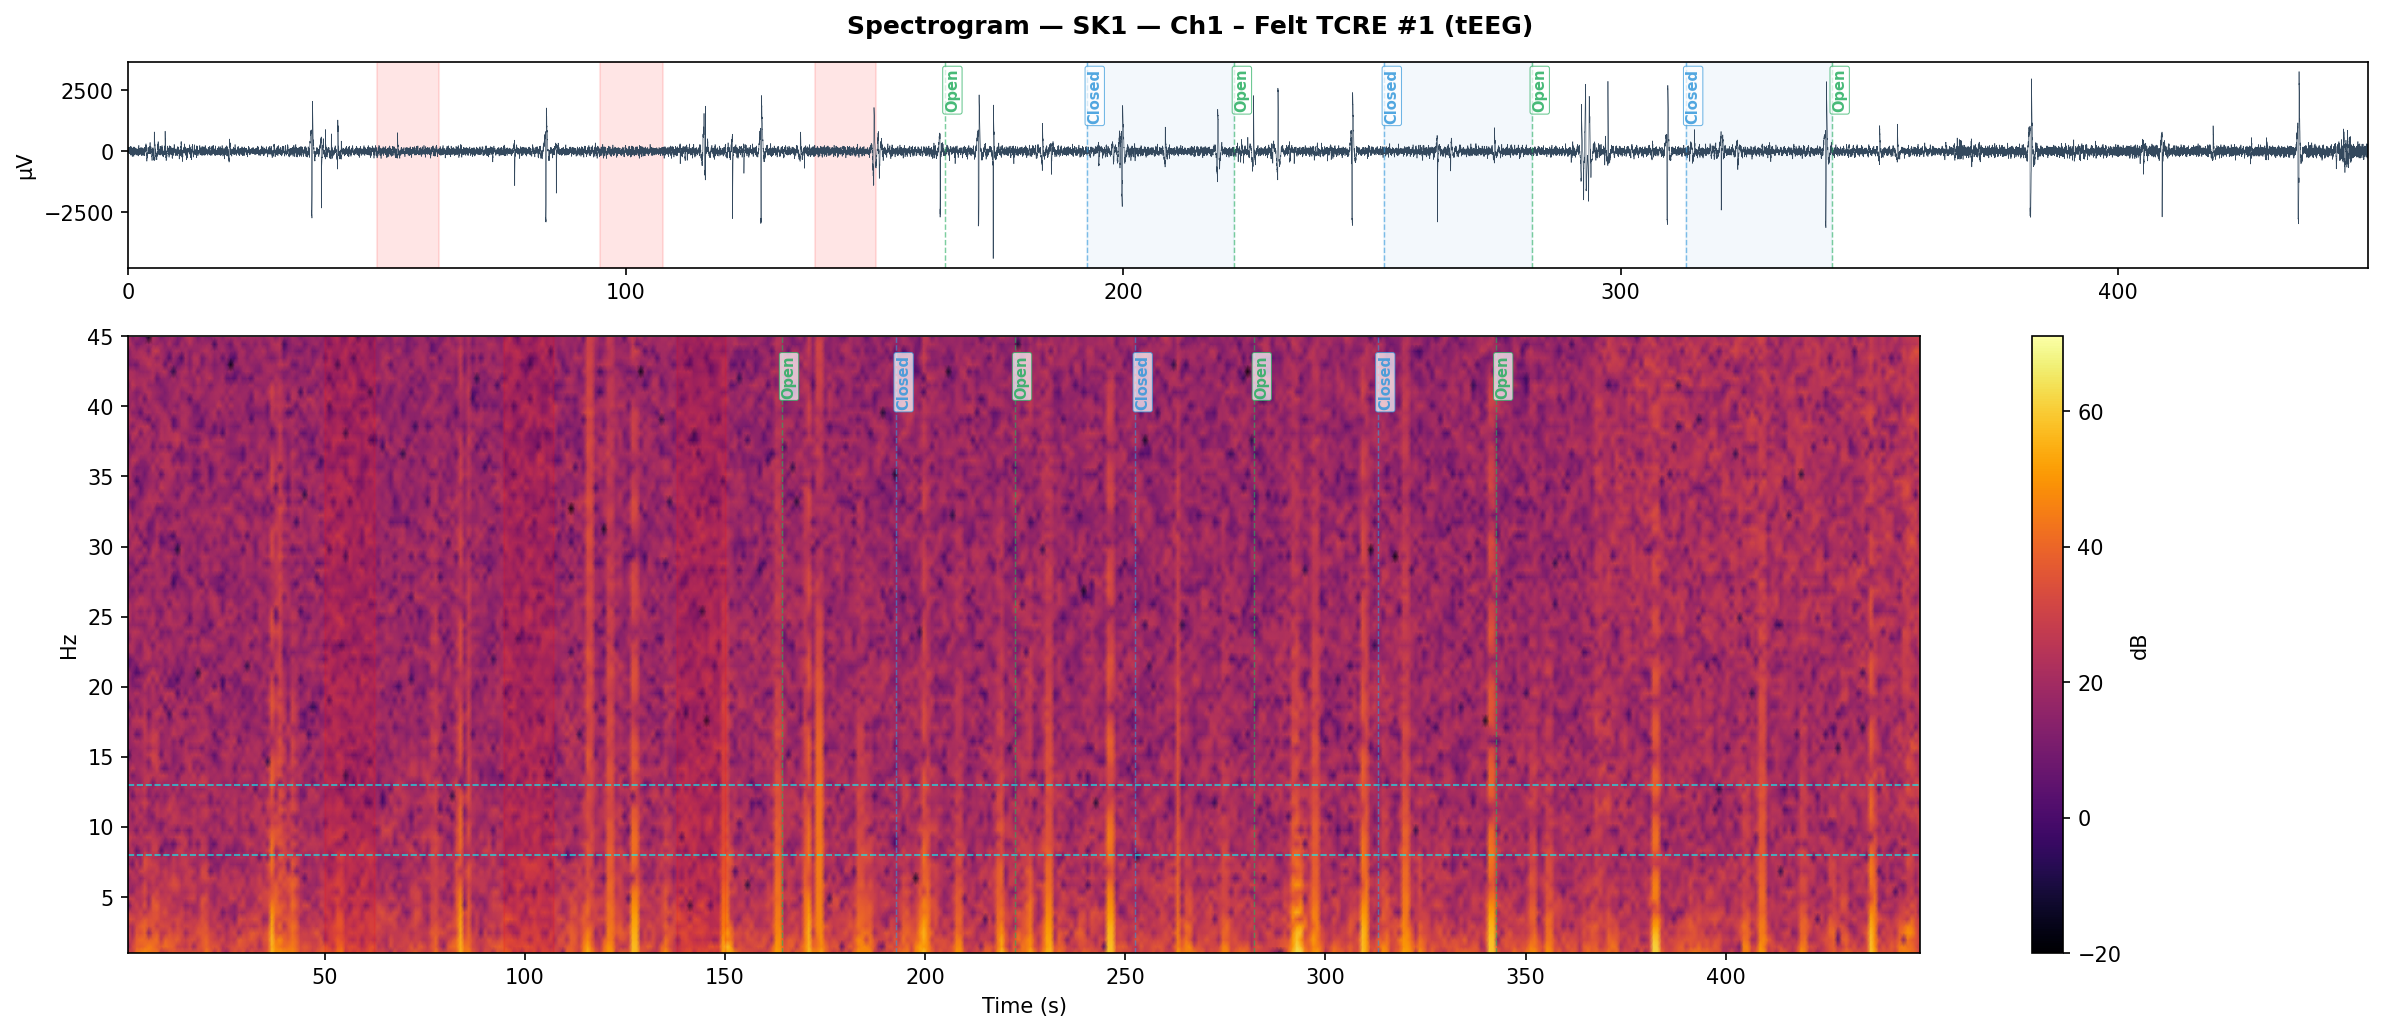
\includegraphics[width=\textwidth]{fig_006.png}
  \caption{Ch1 -- Felt TCRE\,\#1 (tEEG Laplacian). Note the broad
    high-power spectrum consistent with ADC clipping and high impedance.}
  \label{fig:spec_ch1}
\end{figure*}

\begin{figure*}[h]
  \centering
  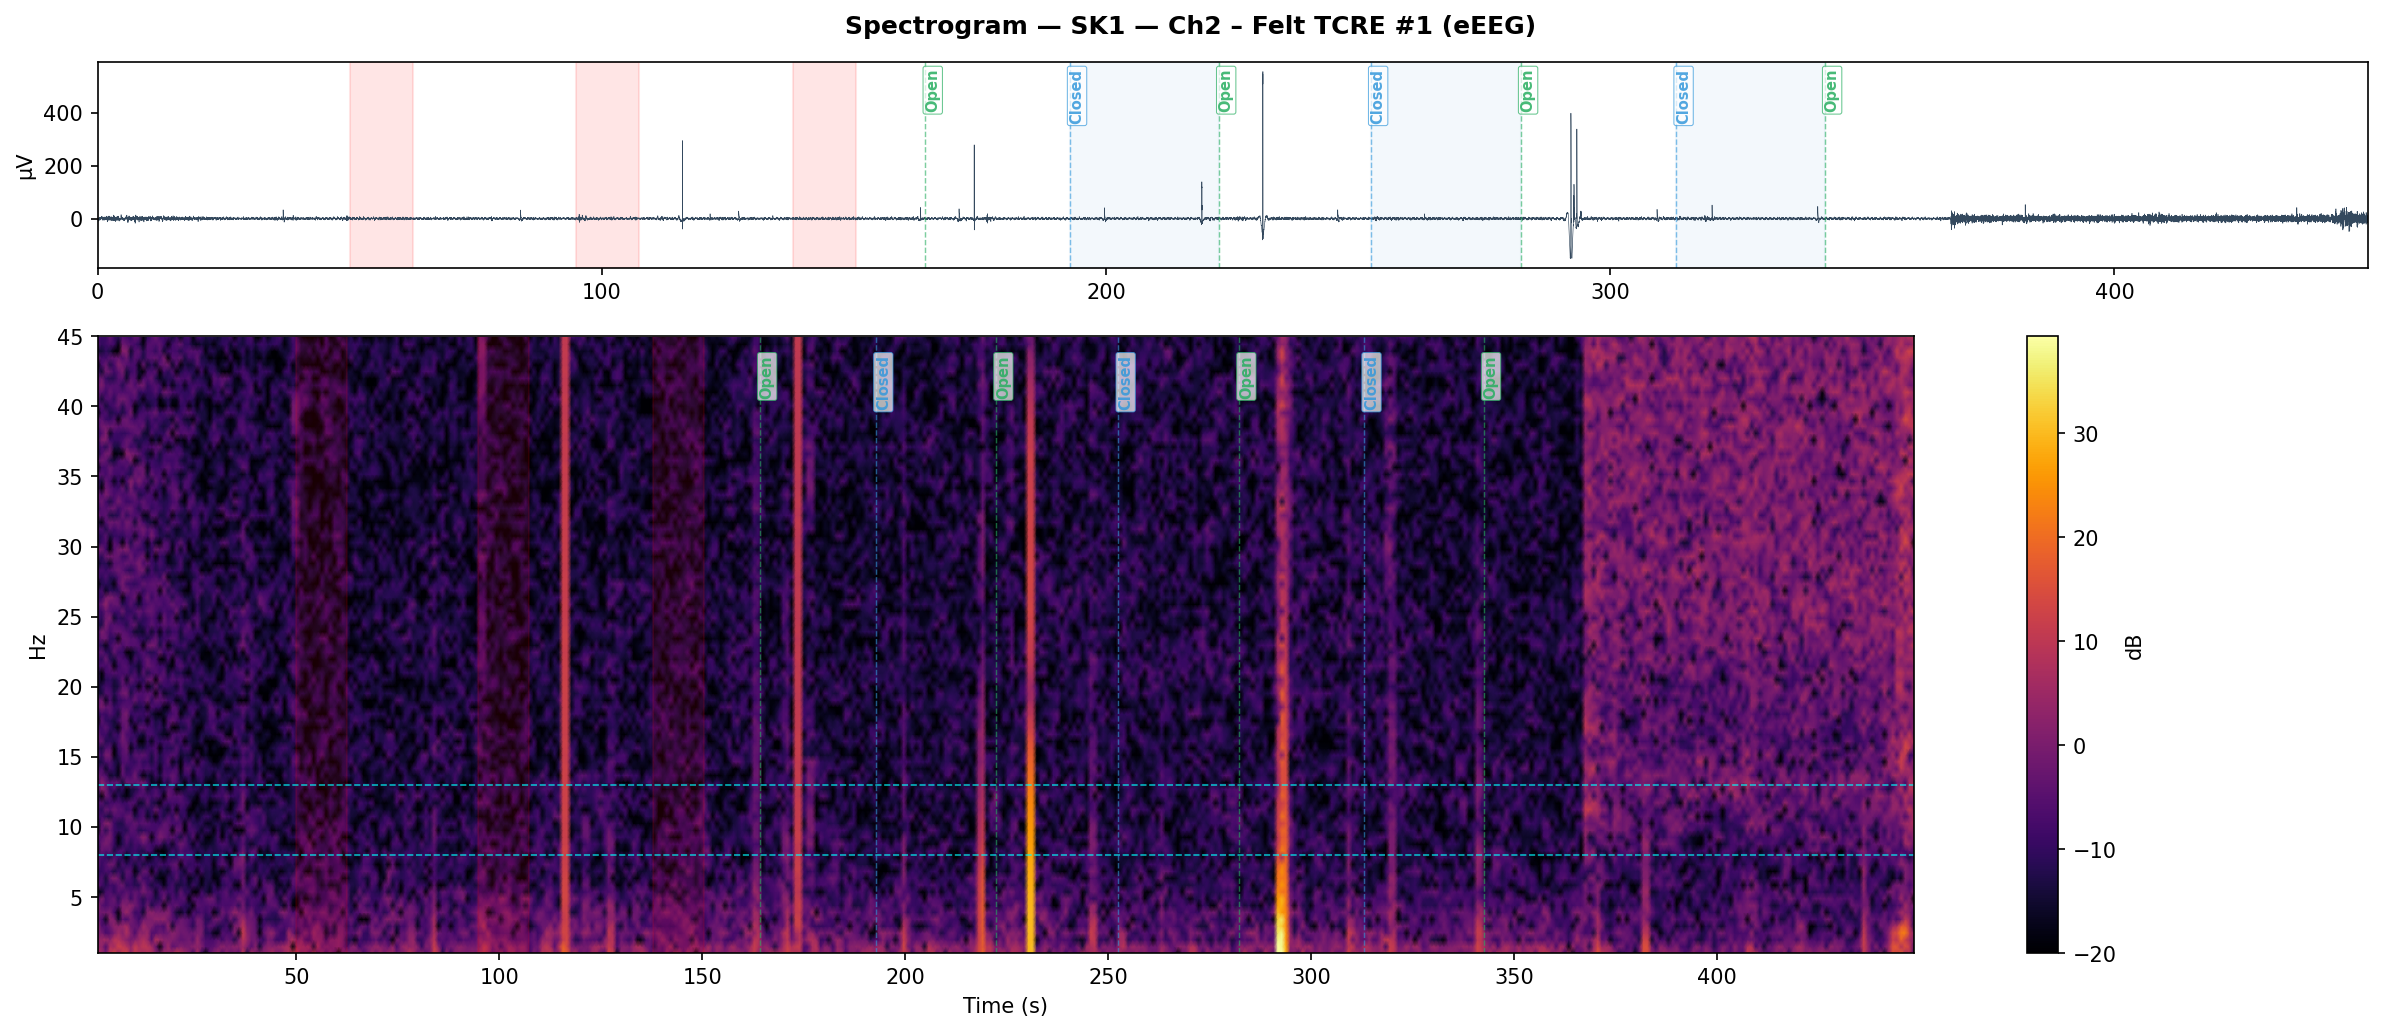
\includegraphics[width=\textwidth]{fig_007.png}
  \caption{Ch2 -- Felt TCRE\,\#1 (eEEG conventional). Much cleaner than
    Ch1; impulse artifacts at stimulus transitions are clearly visible.}
  \label{fig:spec_ch2}
\end{figure*}

\begin{figure*}[h]
  \centering
  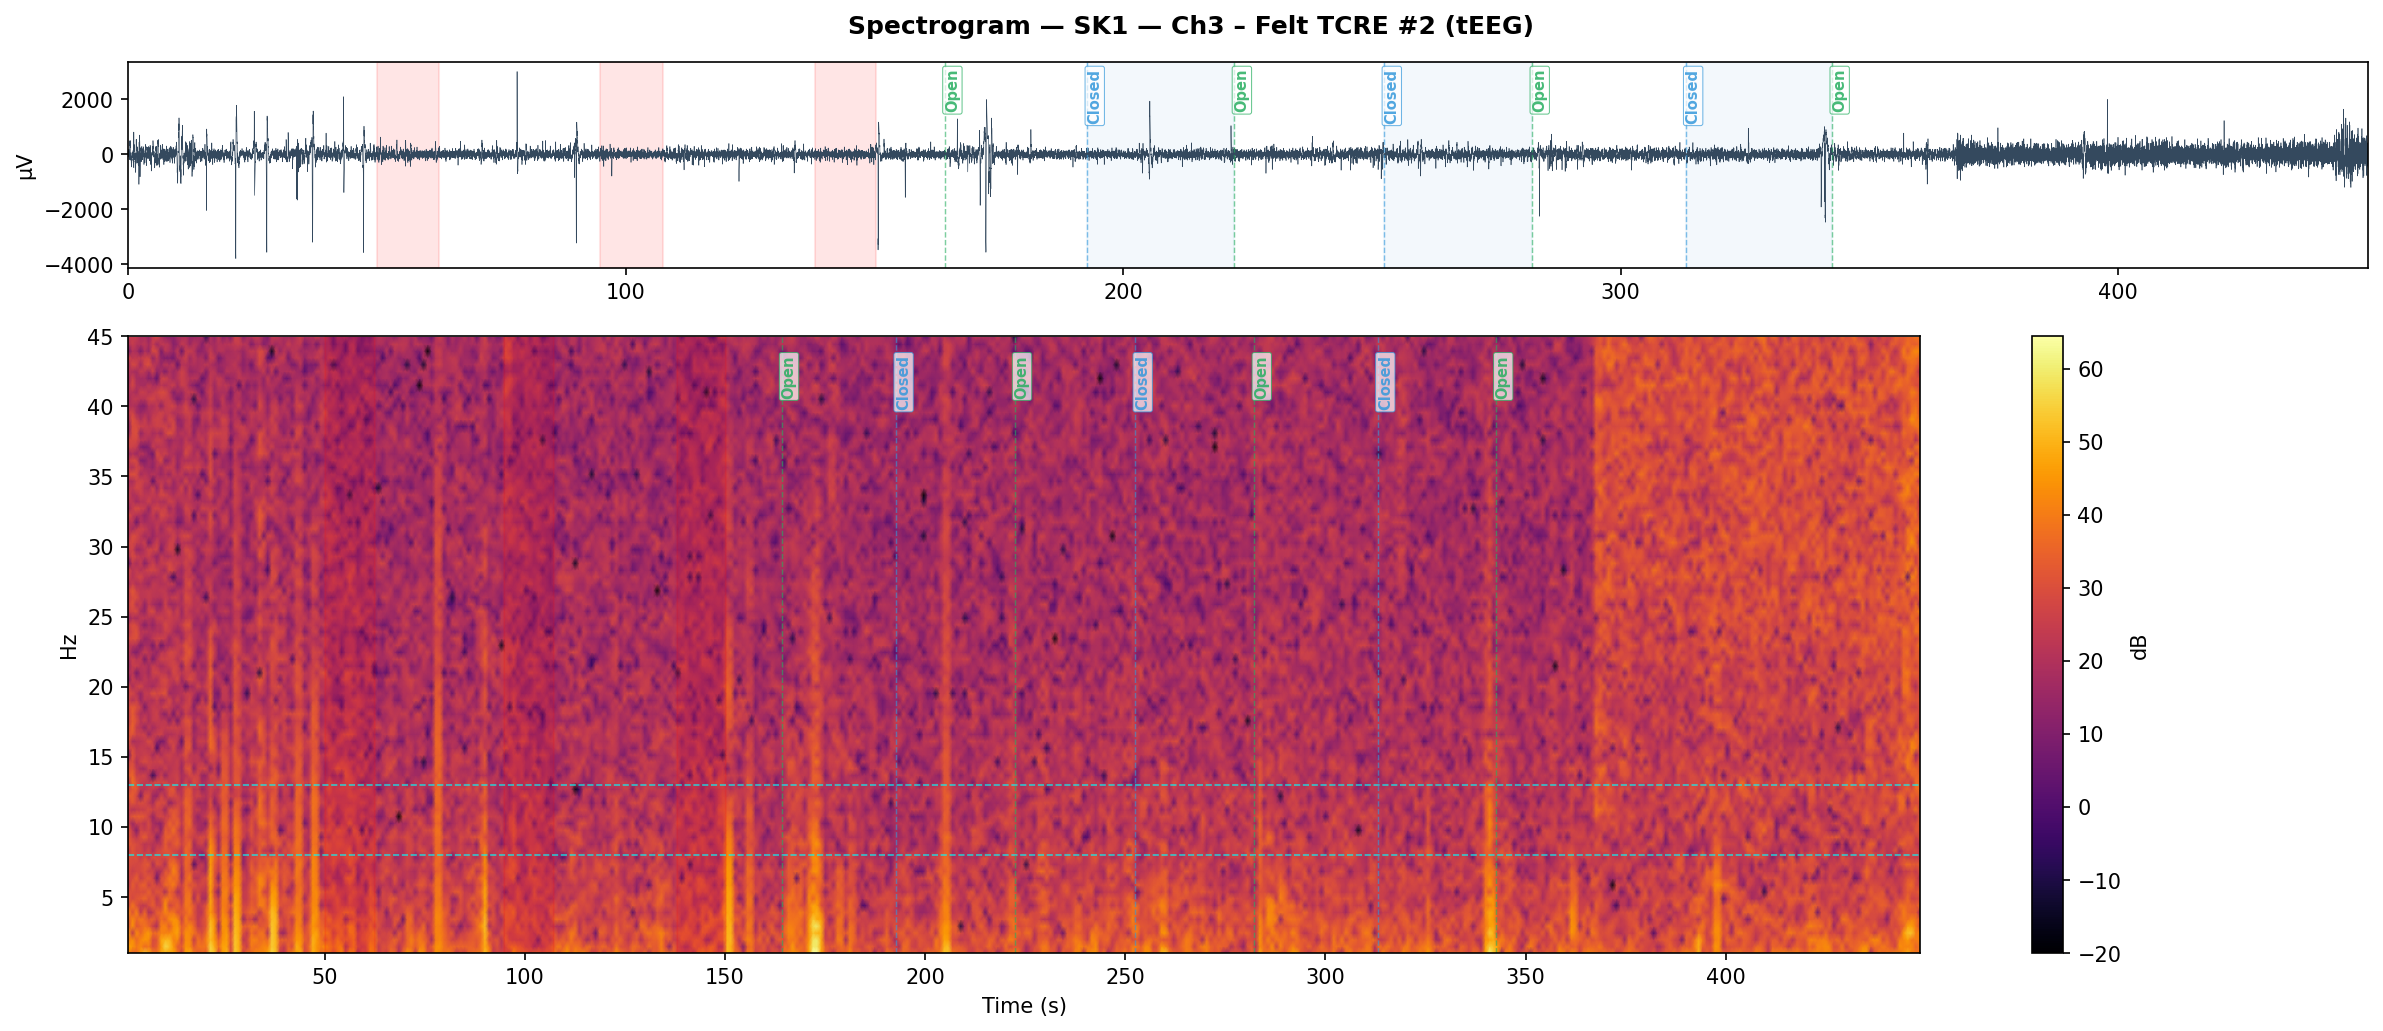
\includegraphics[width=\textwidth]{fig_008.png}
  \caption{Ch3 -- Felt TCRE\,\#2 (tEEG Laplacian). Clipping evident in
    the raw trace; persistent low-frequency energy in the spectrogram.}
  \label{fig:spec_ch3}
\end{figure*}

\begin{figure*}[h]
  \centering
  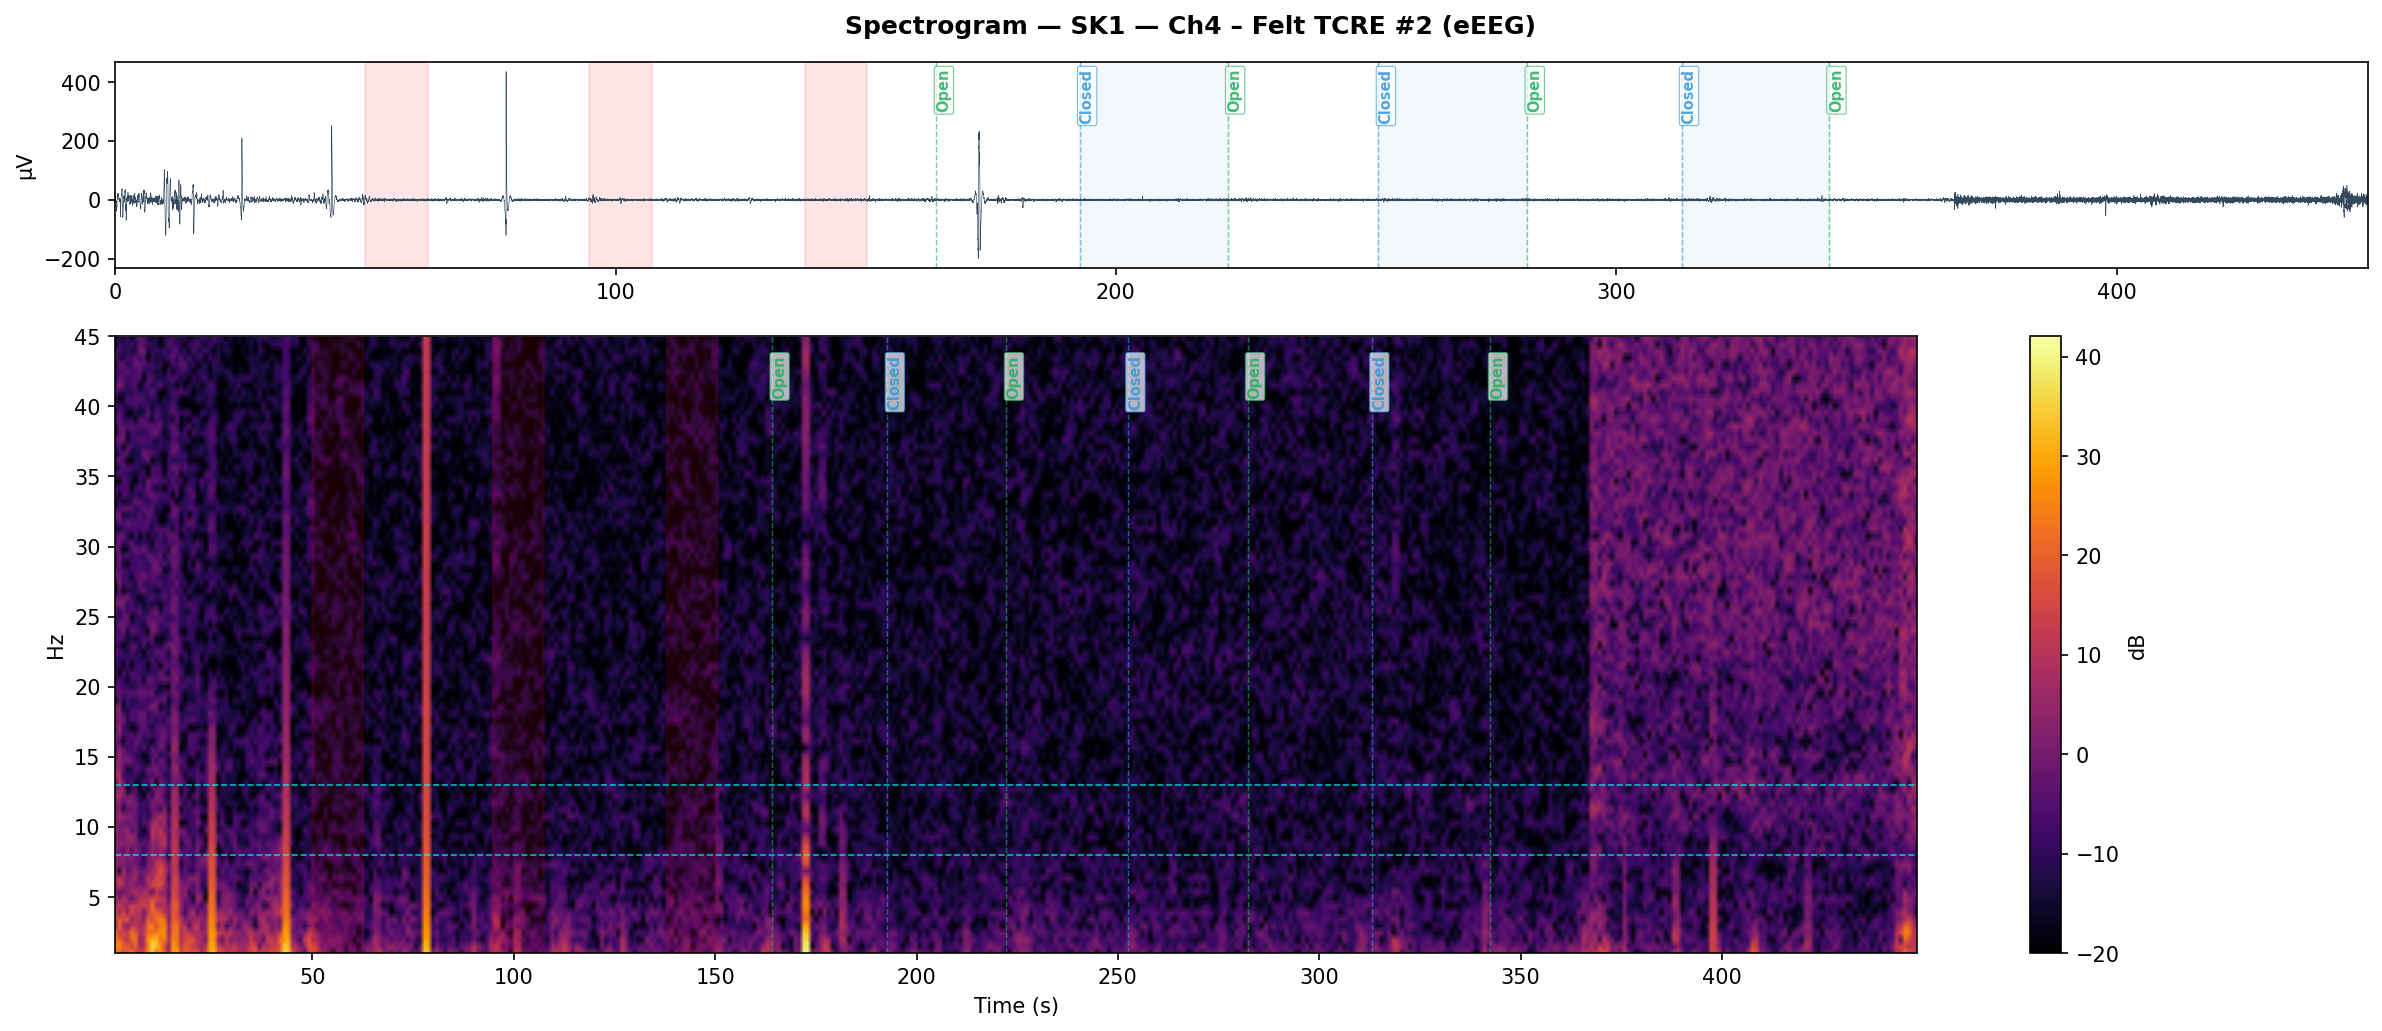
\includegraphics[width=\textwidth]{fig_009.png}
  \caption{Ch4 -- Felt TCRE\,\#2 (eEEG conventional). Clean baseline;
    some residual broadband bursts near stimulus events.}
  \label{fig:spec_ch4}
\end{figure*}

\begin{figure*}[h]
  \centering
  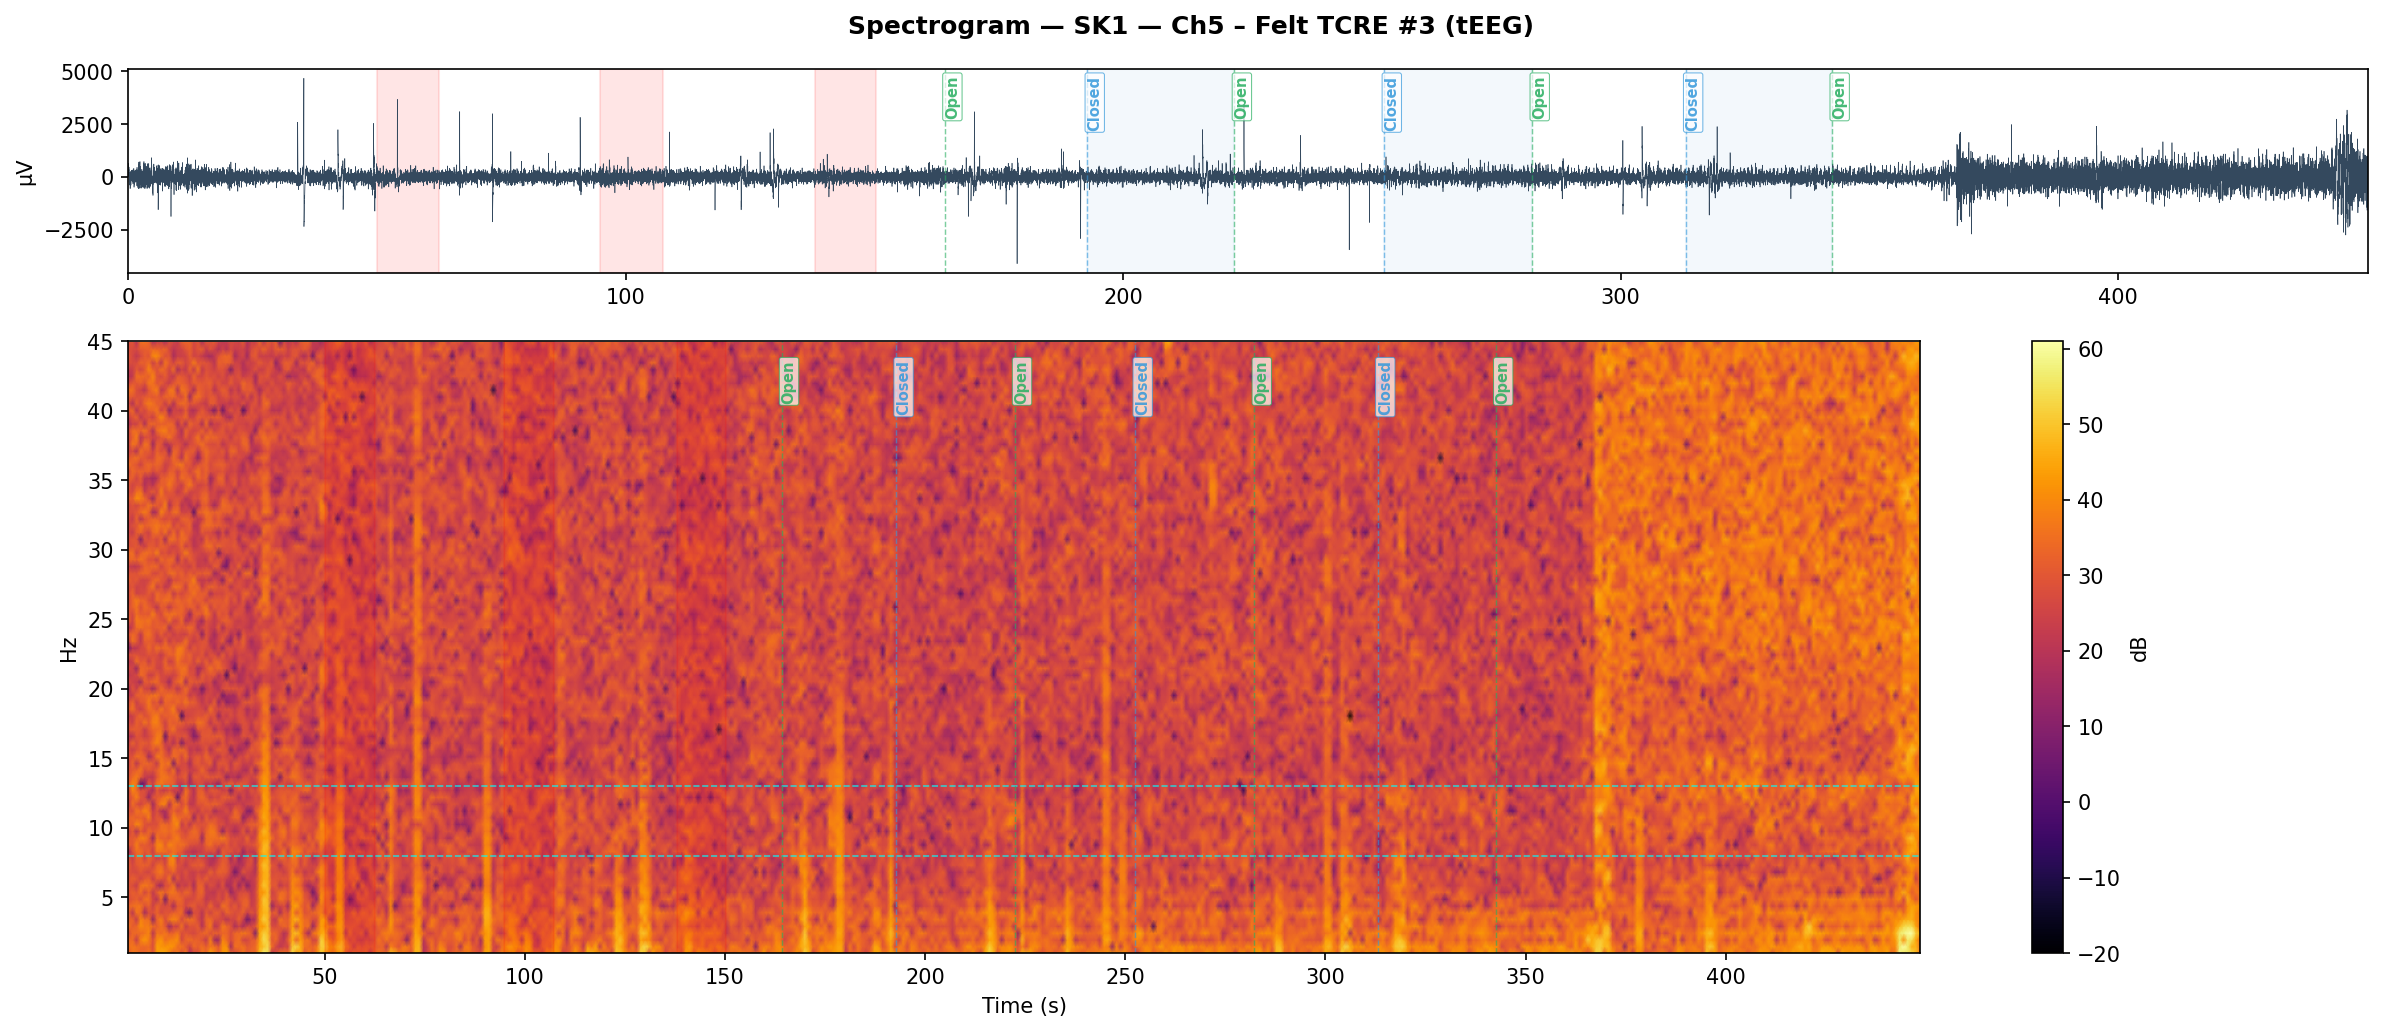
\includegraphics[width=\textwidth]{fig_010.png}
  \caption{Ch5 -- Felt TCRE\,\#3 (tEEG Laplacian). Worst clipping of all
    channels; spectrogram is saturated across all frequencies.}
  \label{fig:spec_ch5}
\end{figure*}

\begin{figure*}[h]
  \centering
  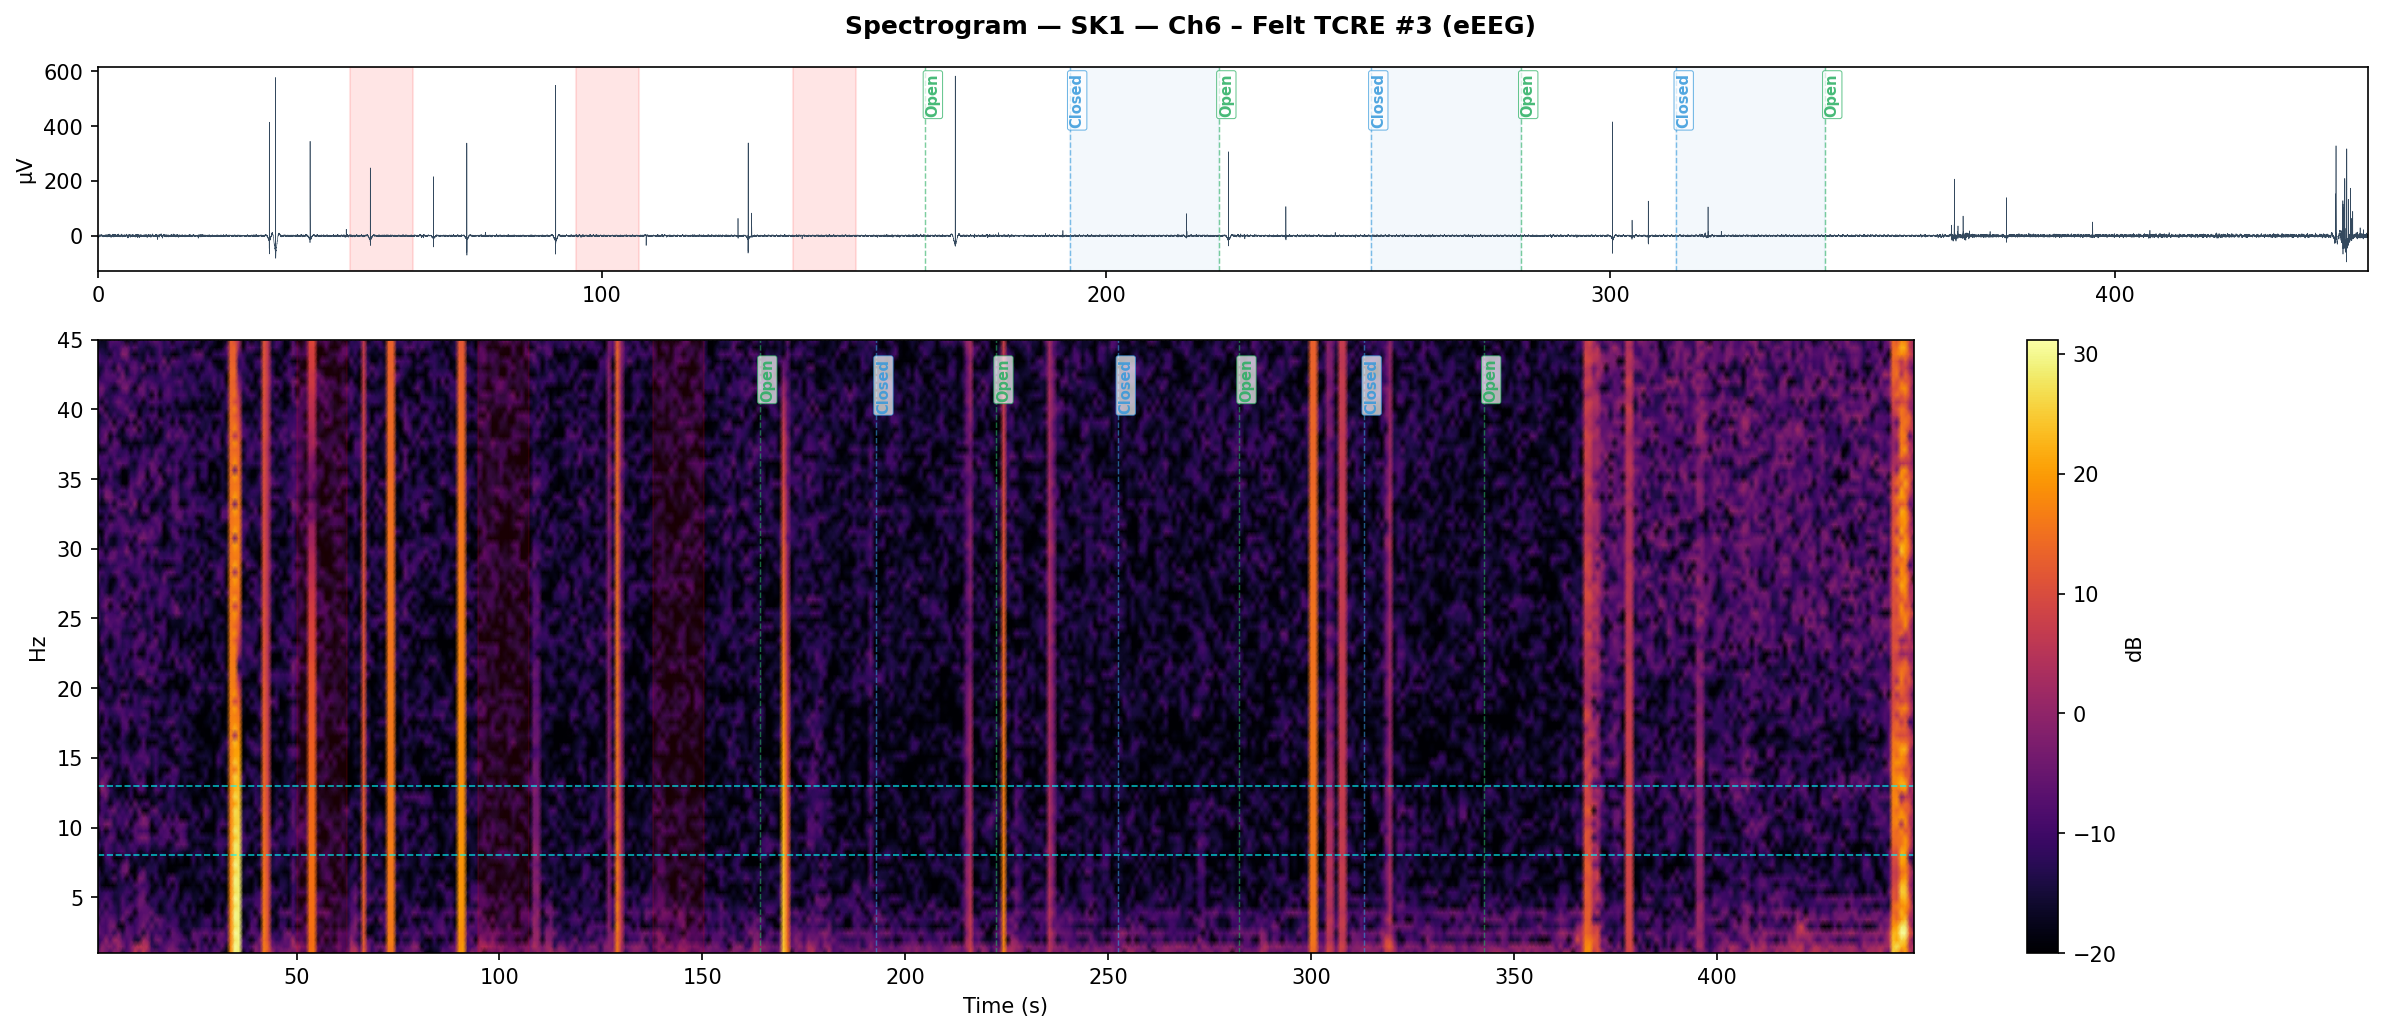
\includegraphics[width=\textwidth]{fig_011.png}
  \caption{Ch6 -- Felt TCRE\,\#3 (eEEG conventional). Very clean signal;
    vertical impulse lines at artifact events are sharp and isolated.}
  \label{fig:spec_ch6}
\end{figure*}

\begin{figure*}[h]
  \centering
  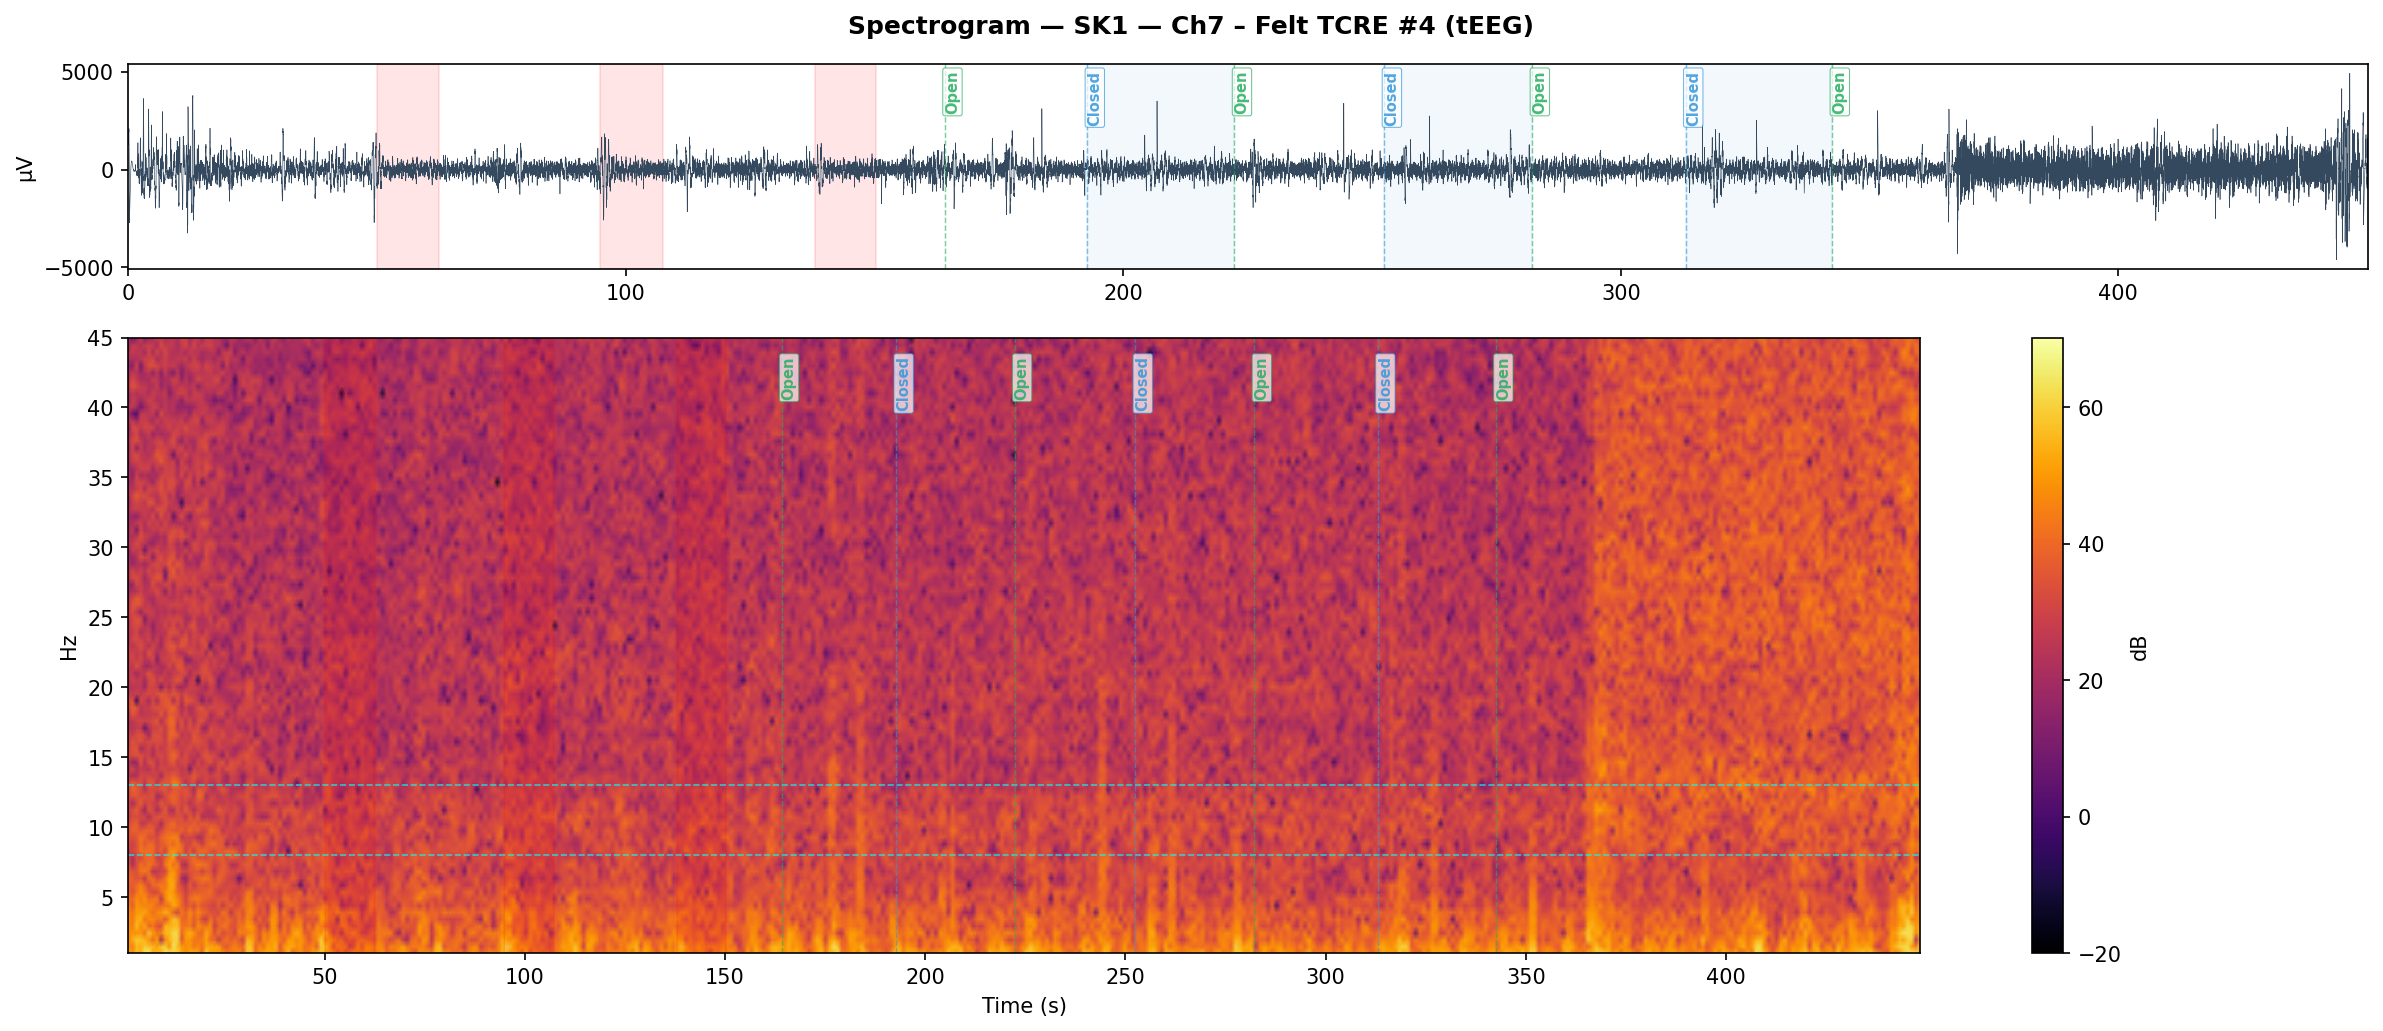
\includegraphics[width=\textwidth]{fig_012.png}
  \caption{Ch7 -- Felt TCRE\,\#4 (tEEG Laplacian). Clipping present but
    slightly less severe than Ch5; broadband noise dominates.}
  \label{fig:spec_ch7}
\end{figure*}

\begin{figure*}[h]
  \centering
  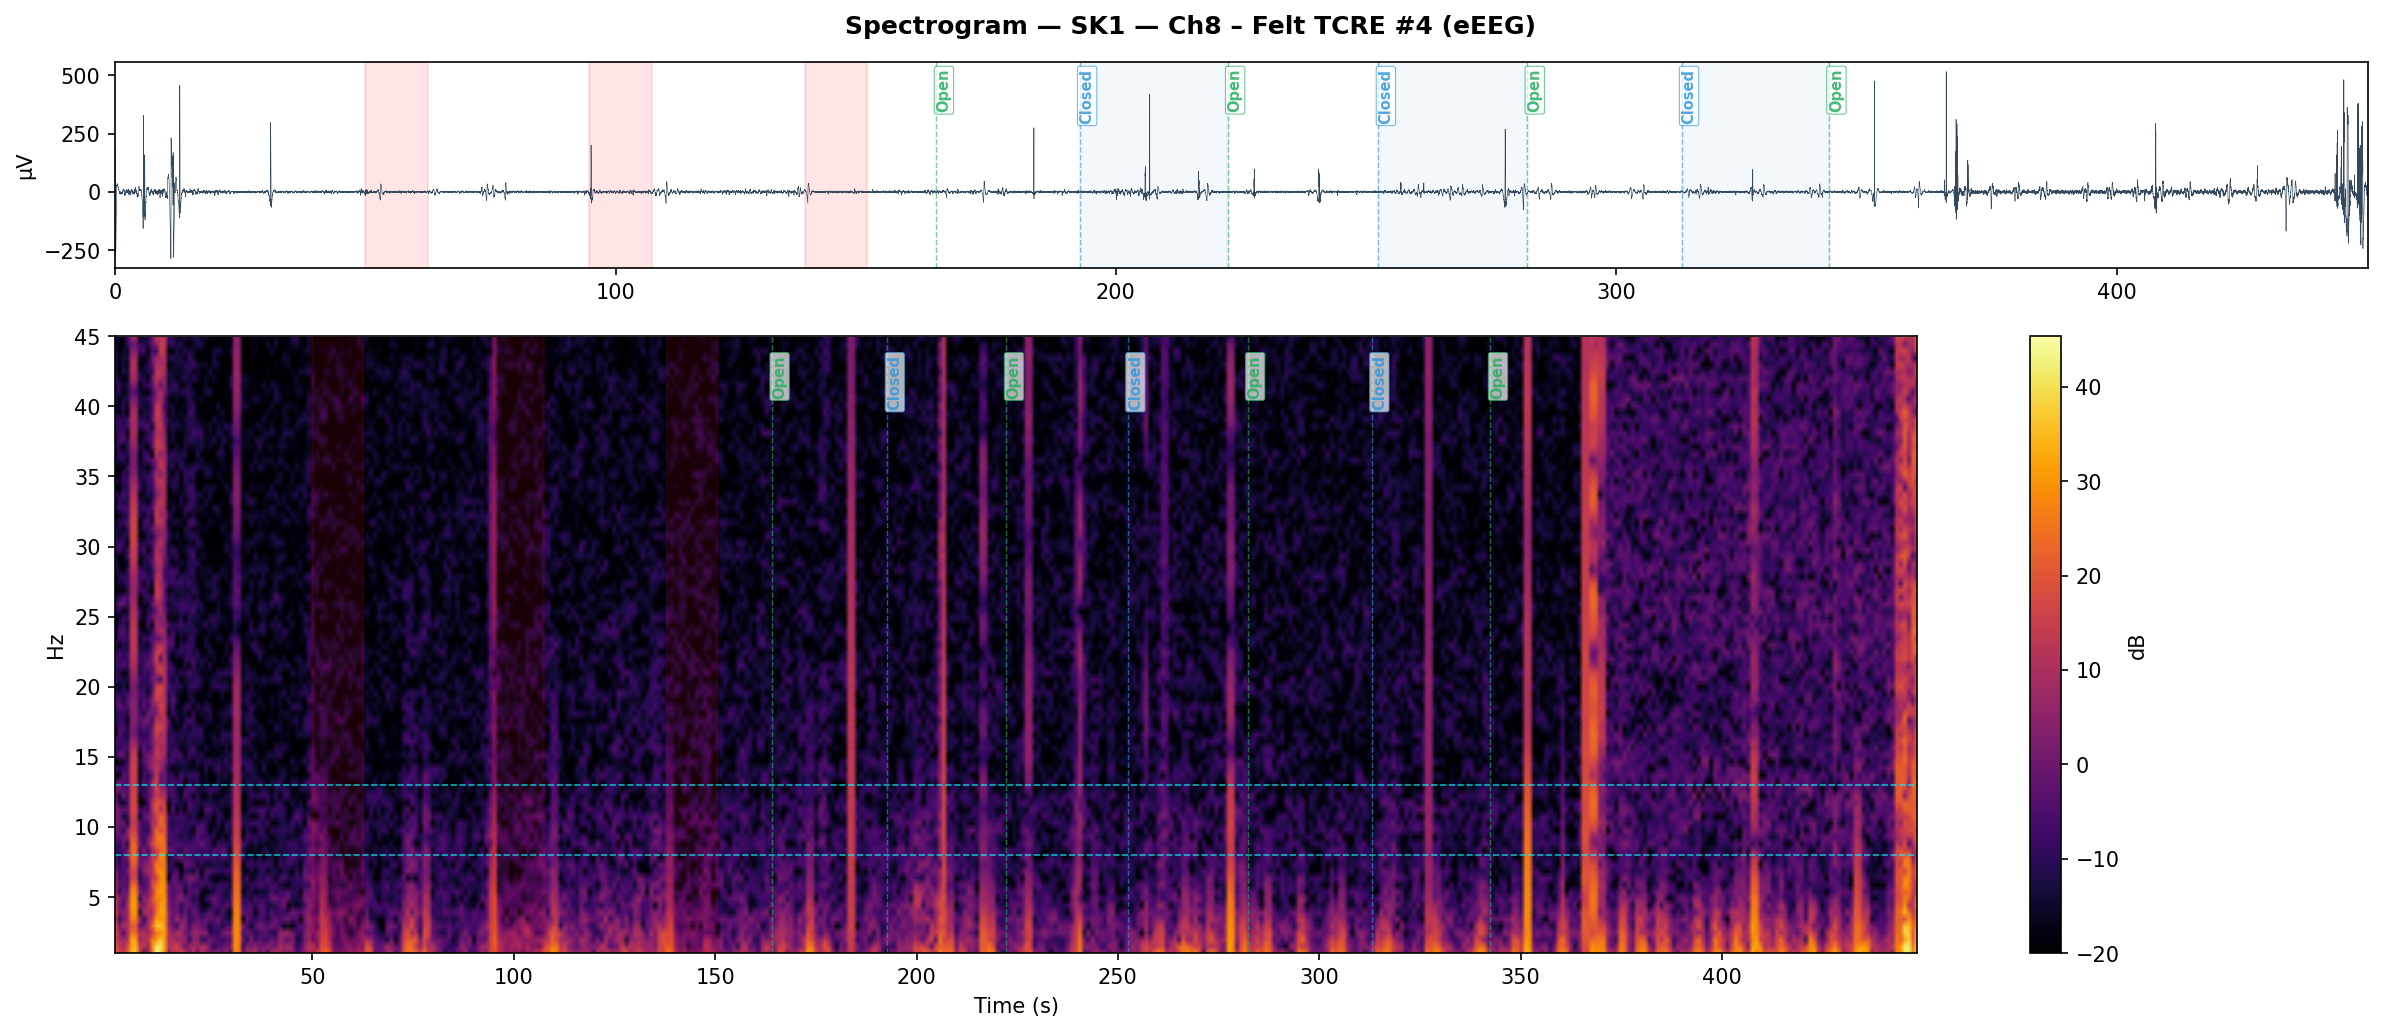
\includegraphics[width=\textwidth]{fig_013.png}
  \caption{Ch8 -- Felt TCRE\,\#4 (eEEG conventional). Clean; alpha-band
    activity faintly visible during some eyes-closed periods.}
  \label{fig:spec_ch8}
\end{figure*}

\begin{figure*}[h]
  \centering
  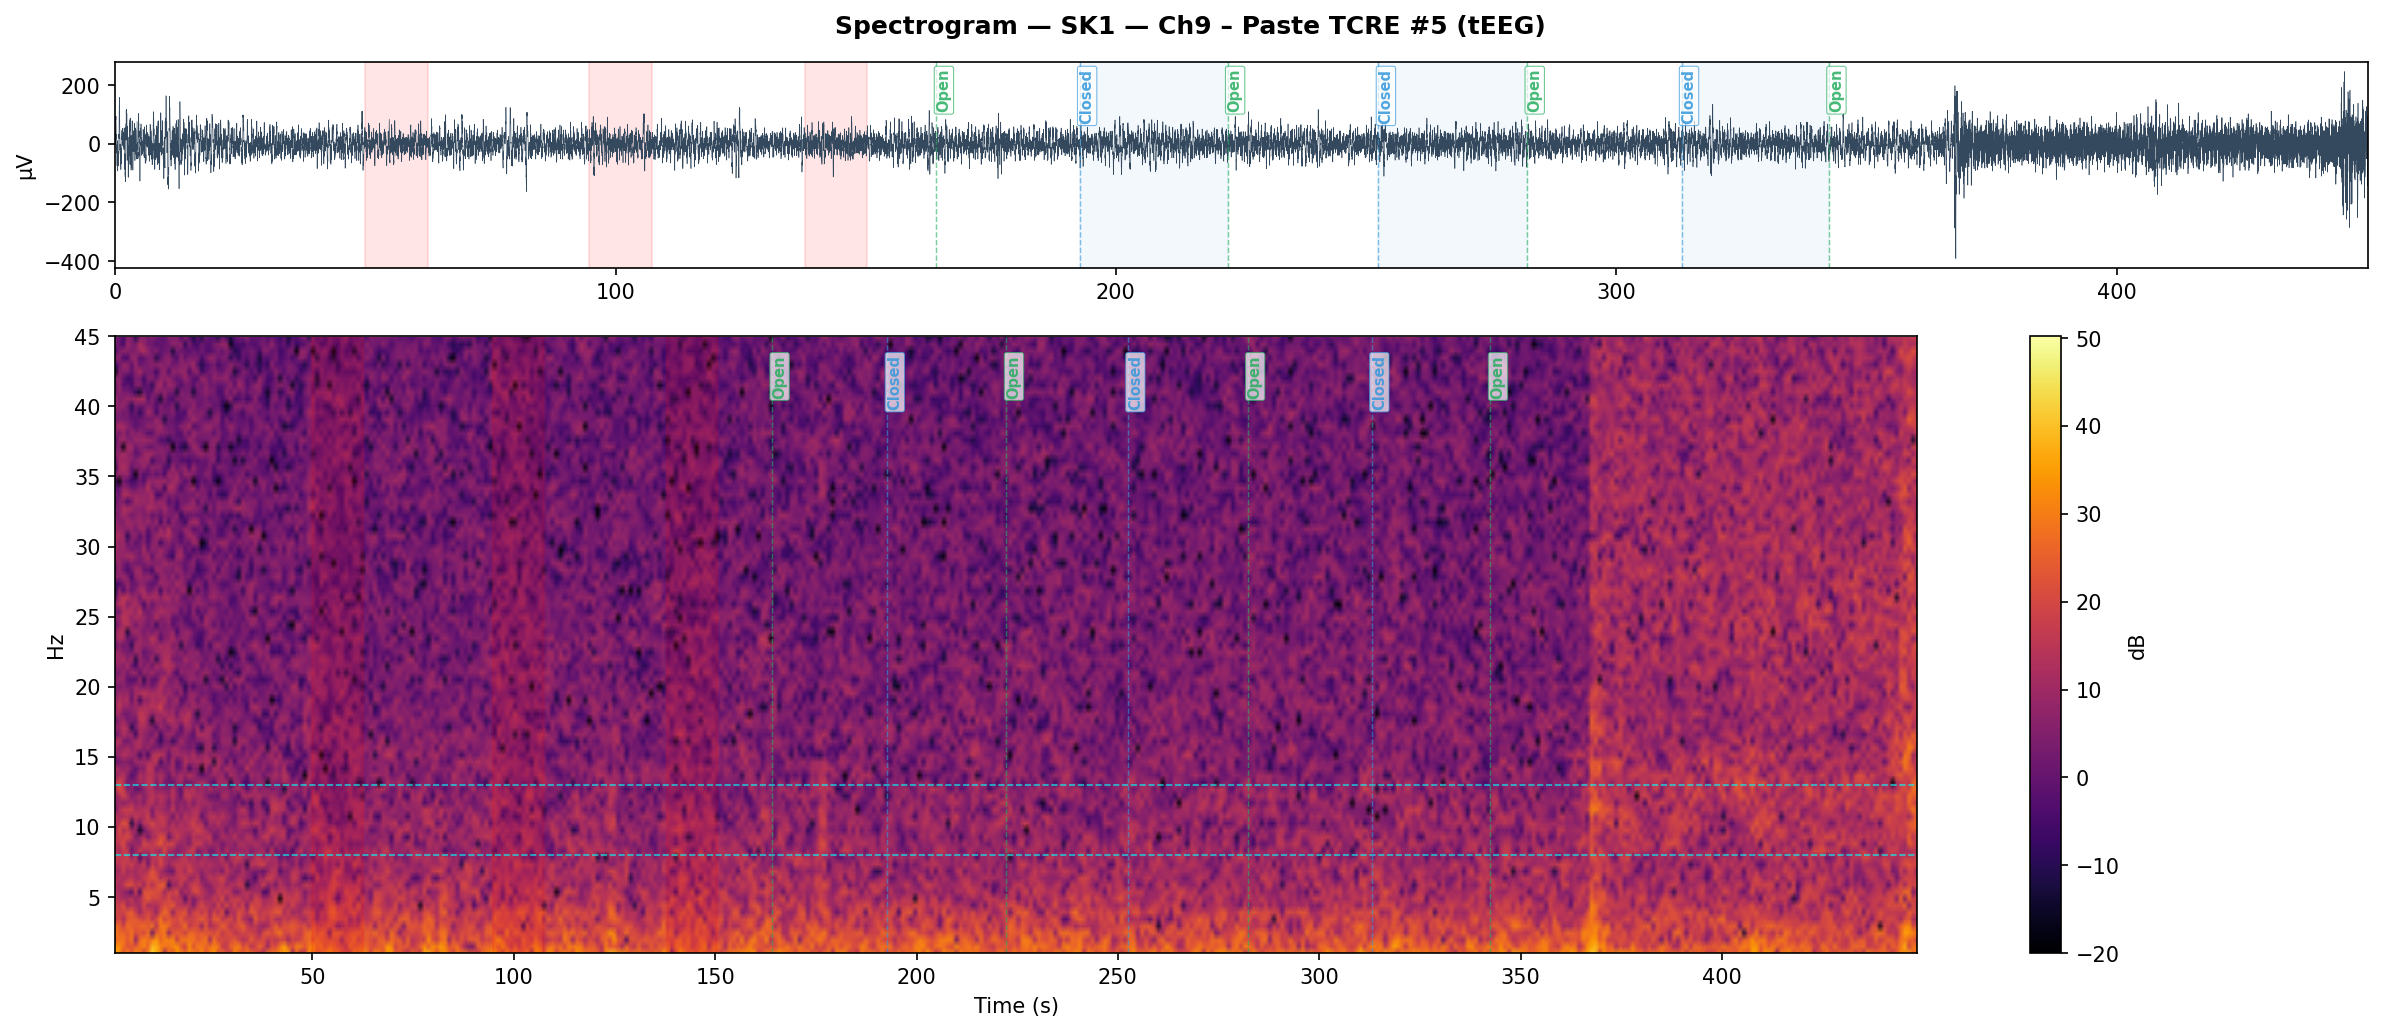
\includegraphics[width=\textwidth]{fig_014.png}
  \caption{Ch9 -- Paste TCRE\,\#5 (tEEG Laplacian). Cleanest tEEG
    channel; low-frequency alpha activity visible in the alpha band during
    resting state.}
  \label{fig:spec_ch9}
\end{figure*}

\begin{figure*}[h]
  \centering
  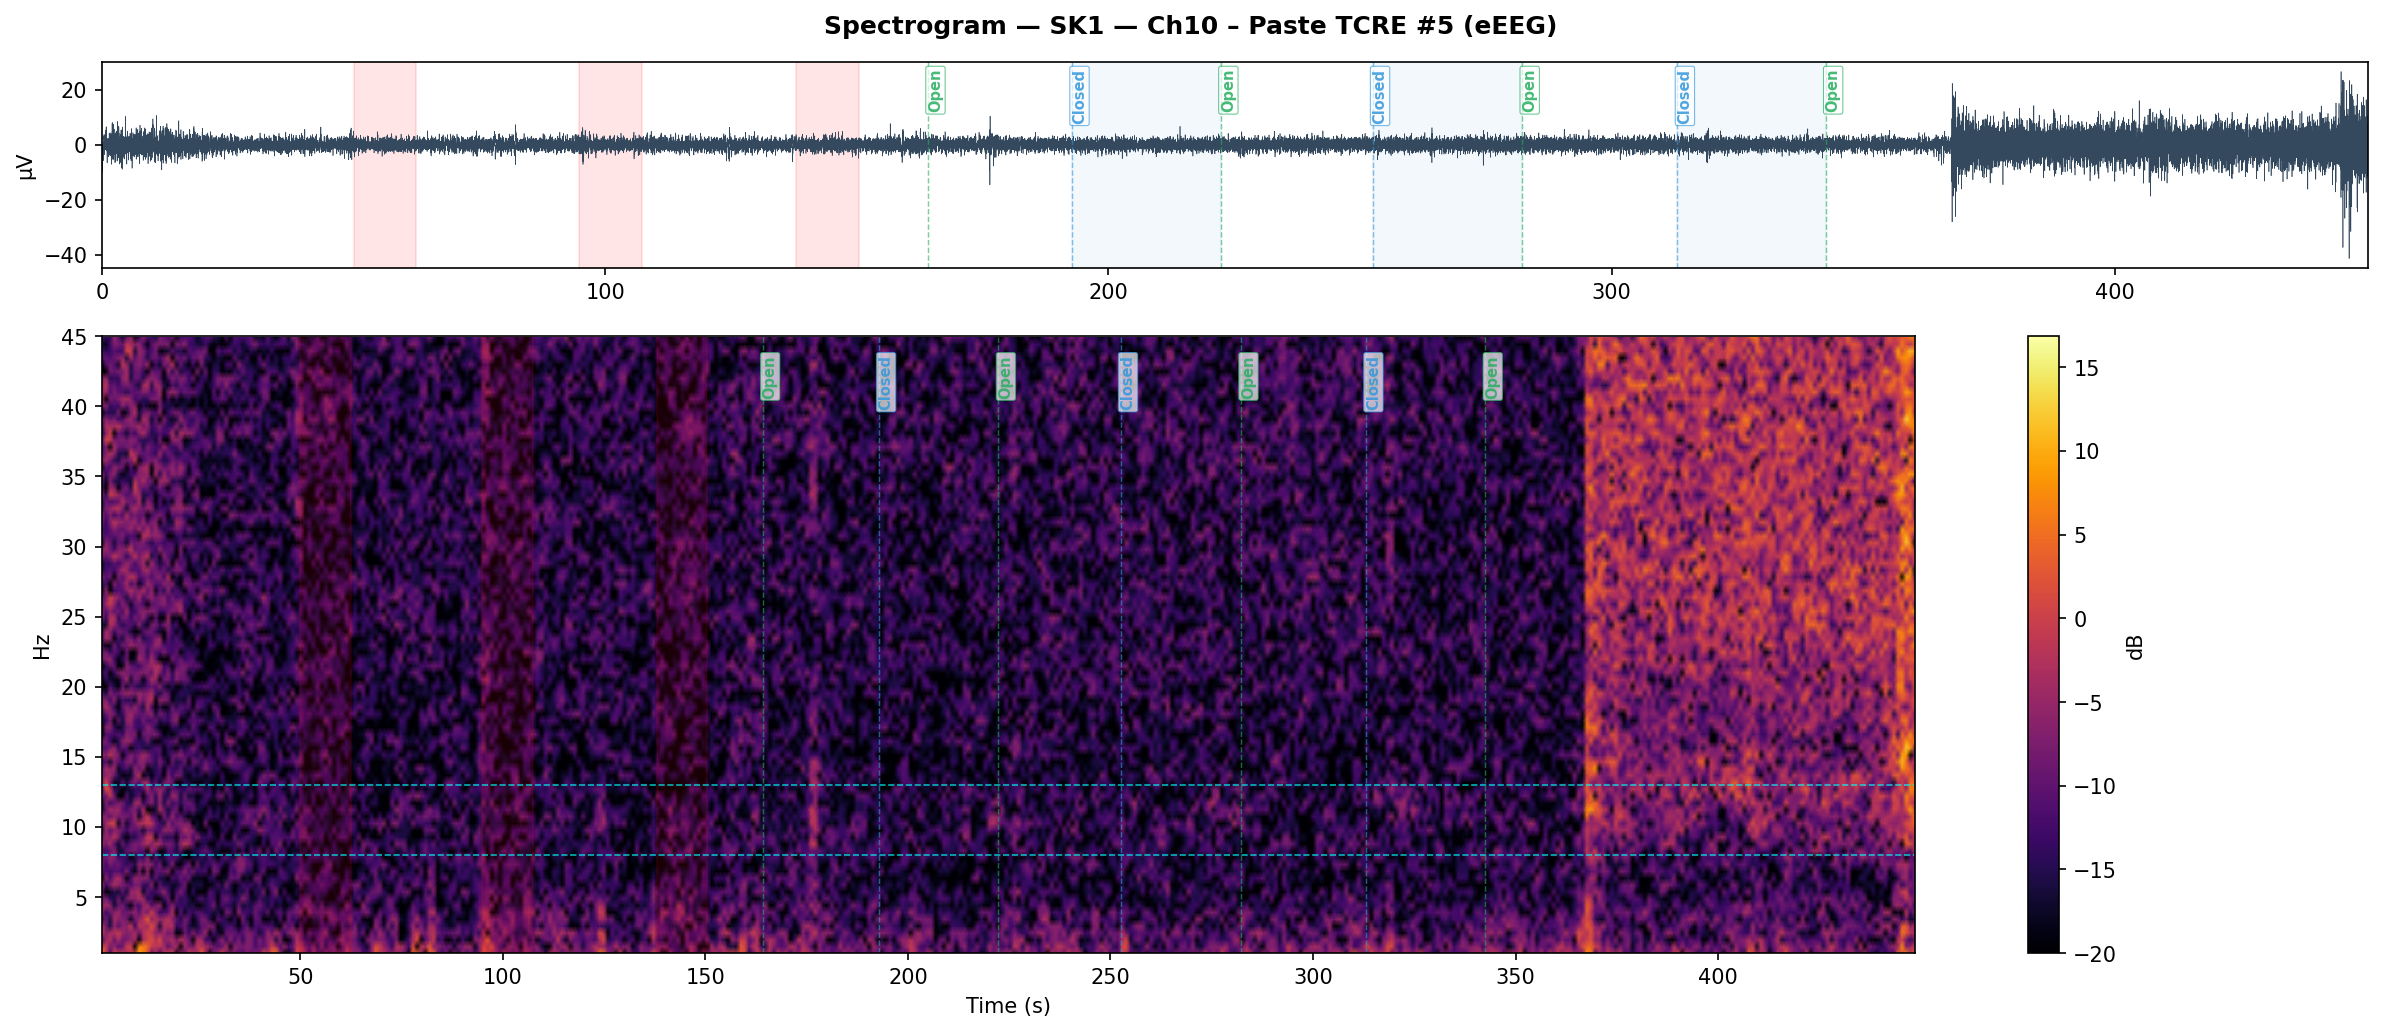
\includegraphics[width=\textwidth]{fig_015.png}
  \caption{Ch10 -- Paste TCRE\,\#5 (eEEG conventional). Cleanest eEEG
    channel overall; very low noise floor with subtle alpha-band activity.}
  \label{fig:spec_ch10}
\end{figure*}

\begin{figure*}[h]
  \centering
  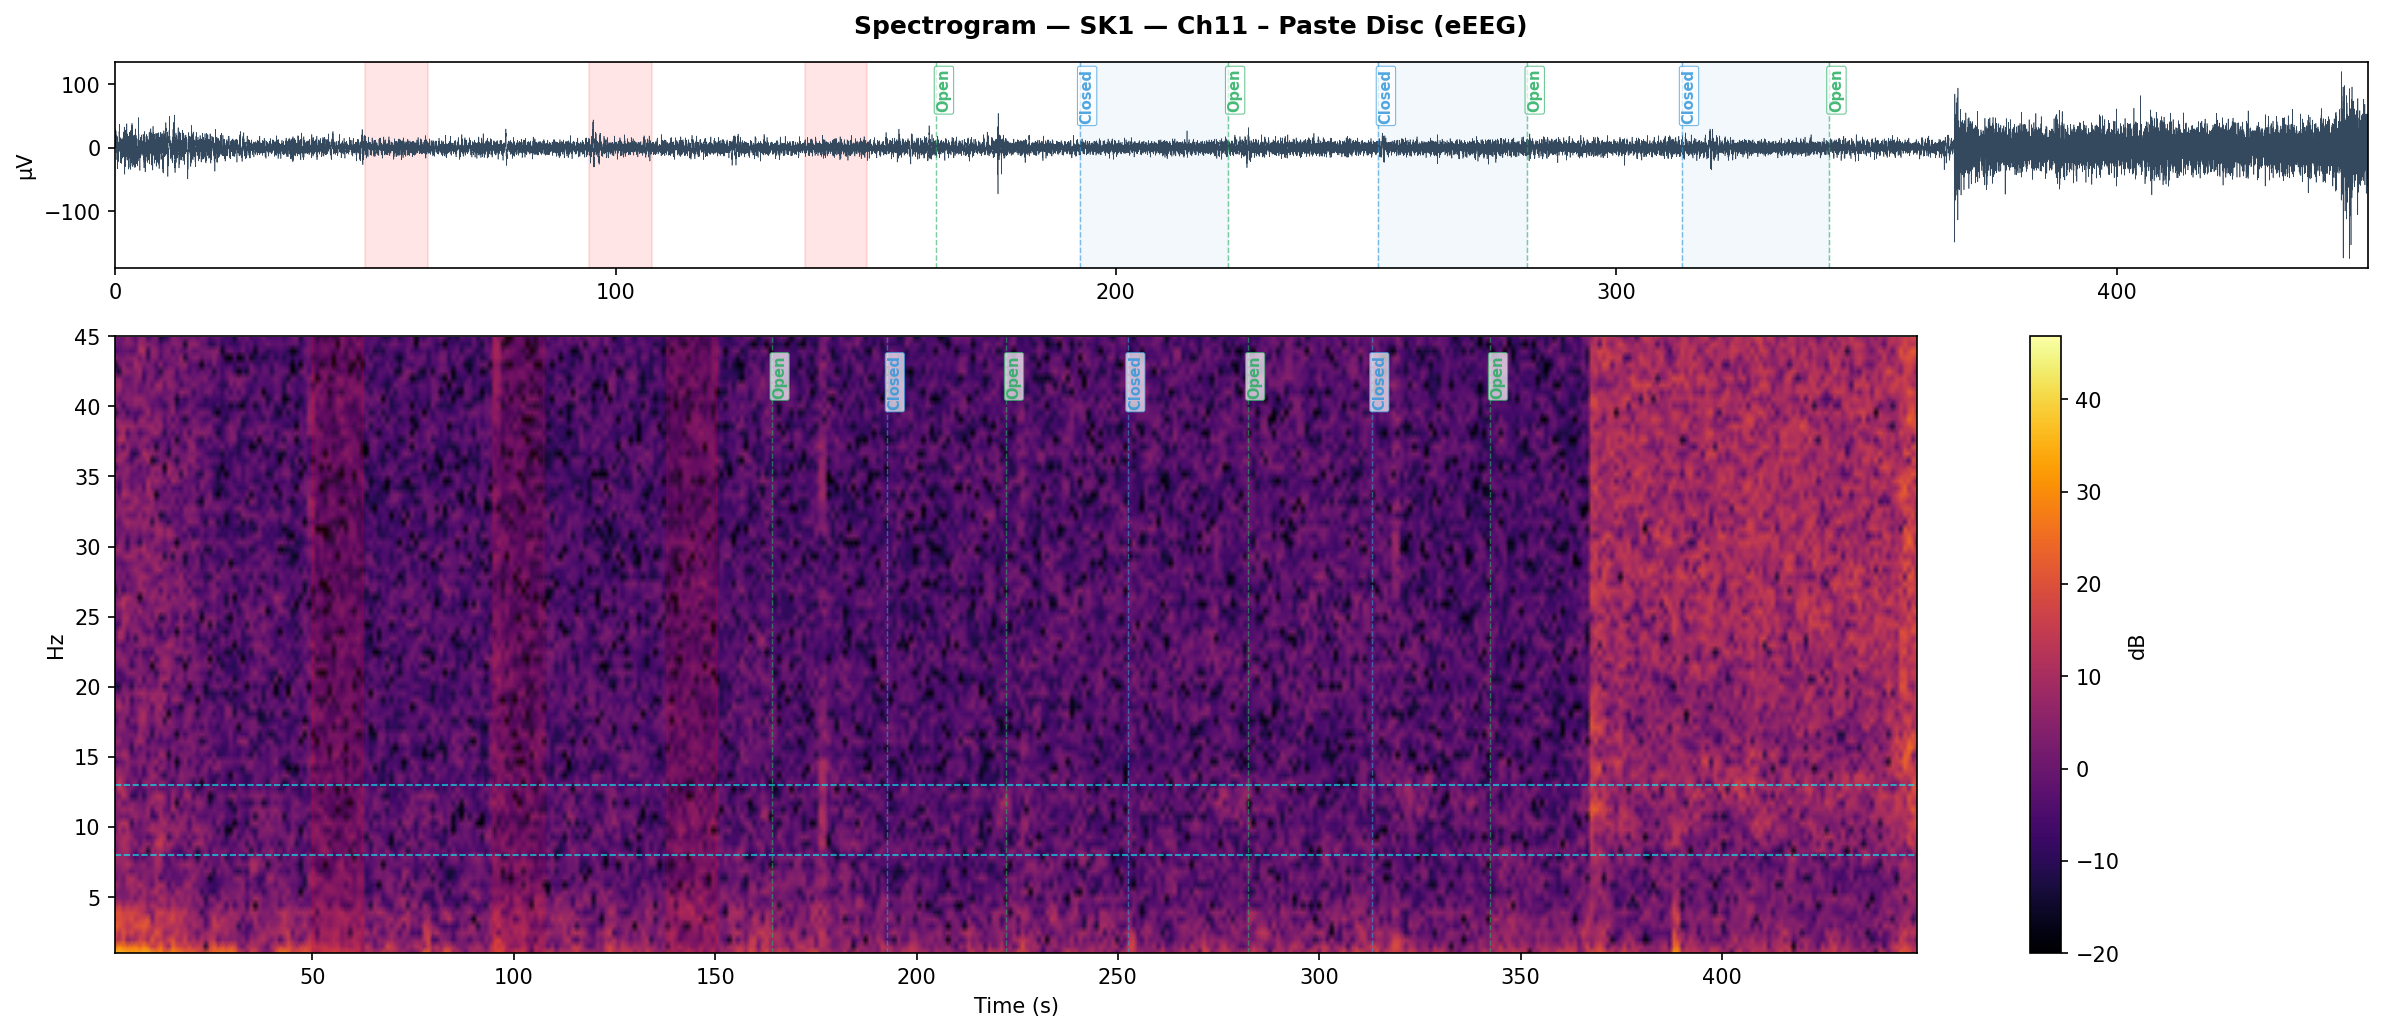
\includegraphics[width=\textwidth]{fig_016.png}
  \caption{Ch11 -- Paste Disc (eEEG). Reference electrode; persistent
    alpha-band energy visible. The large signal drift early in the recording
    is likely a settling artifact from electrode application.}
  \label{fig:spec_ch11}
\end{figure*}

% ─────────────────────────────────────────────────────────────────────────────
%  REFERENCES
% ─────────────────────────────────────────────────────────────────────────────
\begin{thebibliography}{5}

\bibitem{besio2006}
W.~G.~Besio, K.~Koka, R.~Aakula, and W.~Dai,
``Tri-polar concentric ring electrode development for Laplacian
electroencephalography,''
\textit{IEEE Trans.\ Biomed.\ Eng.}, vol.~53, no.~5, pp.~926--933,
May 2006.
doi:~10.1109/TBME.2006.872823.

\bibitem{kirschfeld2005}
K.~Kirschfeld,
``The physical basis of alpha waves in the electroencephalogram and the
origin of the `Berger effect',''
\textit{Biol.\ Cybern.}, vol.~92, no.~3, pp.~177--185, Mar.\ 2005.
doi:~10.1007/s00422-005-0547-1.

\bibitem{donoghue2020}
T.~Donoghue, M.~Haller, E.~J.~Peterson, P.~Varma, P.~Sebastian,
R.~Gao, T.~Noto, A.~H.~Lara, J.~D.~Wallis, R.~T.~Knight,
A.~Shestyuk, and B.~Voytek,
``Parameterizing neural power spectra into periodic and aperiodic
components,''
\textit{Nature Neurosci.}, vol.~23, no.~12, pp.~1655--1665, Dec.\ 2020.
doi:~10.1038/s41593-020-00744-x.

\bibitem{wang2004}
Z.~Wang, A.~C.~Bovik, H.~R.~Sheikh, and E.~P.~Simoncelli,
``Image quality assessment: From error visibility to structural
similarity,''
\textit{IEEE Trans.\ Image Process.}, vol.~13, no.~4, pp.~600--612,
Apr.\ 2004.
doi:~10.1109/TIP.2003.819861.

\bibitem{welch1967}
P.~Welch,
``The use of fast Fourier transform for the estimation of power spectra:
A method based on time averaging over short, modified periodograms,''
\textit{IEEE Trans.\ Audio Electroacoust.}, vol.~15, no.~2, pp.~70--73,
Jun.\ 1967.
doi:~10.1109/TAU.1967.1161901.

\end{thebibliography}

\end{document}